\documentclass[a4paper,12pt]{article}
\usepackage{datetime}
\usepackage{amsmath, amsthm, amssymb}
\usepackage[dvipsnames]{xcolor}
\usepackage{enumitem}
\usepackage{fancyref}

\usepackage[top=1in,bottom=1in,left=1in,right=1in]{geometry} % 用于设置页面布局
\usepackage{xeCJK} % 用于使用本地字体
\usepackage[super, square, sort&compress]{natbib} % 处理参考文献
\usepackage{titlesec, titletoc} % 设置章节标题及页眉页脚
%\usepackage{xCJKnumb} % 中英文数字转换
\usepackage{amssymb}
\usepackage{amsmath} % 在公式中用\text{文本}输入中文
\usepackage{diagbox}
\usepackage{multirow} % 表格中使用多行
\usepackage{booktabs} % 表格中使用\toprule等命令
\usepackage{rotating} % 使用sidewaystable环境旋转表格
\usepackage{tabularx}
\usepackage{graphicx} % 处理图片
\usepackage{footnote} % 增强的脚注功能,可添加表格脚注
\usepackage{threeparttable} % 添加真正的表格脚注,示例见README
\usepackage{hyperref} % 添加pdf书签

\usepackage{tikz}
\usetikzlibrary{shapes,arrows,shadows}

% 字体设置
\setmainfont{Times New Roman}
\setsansfont[Scale=MatchLowercase,Mapping=tex-text]{PT Sans}
\setmonofont[Scale=MatchLowercase]{PT Mono}
\setCJKmainfont[ItalicFont={Kaiti SC}, BoldFont={Heiti SC}]{Songti SC}
\setCJKsansfont{Heiti SC}
\setCJKmonofont{Songti SC}
% \setCJKmainfont[BoldFont={FZXiaoBiaoSong-B05S}]{Songti SC}
% \setCJKfamilyfont{kai}[BoldFont=Heiti SC]{Kaiti SC}
% \setCJKfamilyfont{song}[BoldFont=Heiti SC]{Songti SC}
% \setCJKfamilyfont{hei}[BoldFont=Heiti SC]{Heiti SC}
% \setCJKfamilyfont{fsong}[BoldFont=Heiti SC]{Songti SC}
% \newcommand{\kai}[1]{{\CJKfamily{kai}#1}}
% \newcommand{\hei}[1]{{\CJKfamily{hei}#1}}
% \setromanfont[Mapping=tex-text]{TeXGyrePagella}
% \setsansfont[Scale=MatchLowercase,Mapping=tex-text]{TeXGyrePagella}
% \setmonofont[Scale=MatchLowercase]{Courier New}
%%设置常用中文字号,方便调用
\newcommand{\erhao}{\fontsize{22pt}{\baselineskip}\selectfont}
\newcommand{\xiaoerhao}{\fontsize{18pt}{\baselineskip}\selectfont}
\newcommand{\sanhao}{\fontsize{16pt}{\baselineskip}\selectfont}
\newcommand{\xiaosanhao}{\fontsize{15pt}{\baselineskip}\selectfont}
\newcommand{\sihao}{\fontsize{14pt}{\baselineskip}\selectfont}
\newcommand{\xiaosihao}{\fontsize{12pt}{\baselineskip}\selectfont}
\newcommand{\wuhao}{\fontsize{10.5pt}{\baselineskip}\selectfont}
\newcommand{\xiaowuhao}{\fontsize{9pt}{\baselineskip}\selectfont}
\newcommand{\liuhao}{\fontsize{7.5pt}{\baselineskip}\selectfont}

% 章节标题显示方式及页眉页脚设置
% \item xCJKnumb是自己额外安装的包
% \item titleformat命令定义标题的形式
% \item titlespacing定义标题距左、上、下的距离
\titleformat{\section}{\raggedright\large\bfseries}{\thesection}{1em}{}
\titleformat{\subsection}{\raggedright\normalsize\bfseries}{\thesubsection}{1em}{}
\titlespacing{\section}{0pt}{*0}{*2}
\titlespacing{\subsection}{0pt}{*0}{*1}
% 由于默认的2em缩进不够,所以我手动调整了,但是在windows下似乎2.2就差不多了,或者是article中没有这个问题
\setlength{\parindent}{2.2em}

% 设置表格标题前后间距
\setlength{\abovecaptionskip}{0pt}
\setlength{\belowcaptionskip}{0pt}


\renewcommand{\refname}{\bfseries{参~考~文~献}} %将Reference改为参考文献(用于 article)
% \renewcommand{\bibname}{参~考~文~献} %将bibiography改为参考文献(用于 book)
\renewcommand{\baselinestretch}{1.38} %设置行间距
\renewcommand{\figurename}{\small\ttfamily 图}
\renewcommand{\tablename}{\small\ttfamily 表}


\setlength{\parindent}{0em}

\newcommand{\specialcell}[2][c]{%
  \begin{tabular}[#1]{@{}c@{}}#2\end{tabular}}

\newtheorem{definition}{定义}
\newtheorem{lemma}{引理}
\newtheorem{proposition}{命题}
\newtheorem{grammar}{文法}
\newtheorem{program}{程序}
\newtheorem{convention}{约定}
\renewcommand*{\proofname}{证明}

\usetikzlibrary{shapes.geometric}
\tikzset{
    turtle/.style={
        draw,
        shape border rotate=270,
        regular polygon,
        regular polygon sides=3,
        fill=gray,
        node distance=2cm,
        minimum height=4em
    }
}

\newdateformat{monthyeardate}{\THEYEAR 年 \THEMONTH 月}

\title{在庞加莱圆盘上看加法与乘法}
\author{苑明理}
\date{\monthyeardate\today}

\begin{document}

\begin{center}
  \sihao \em 过程比结果更重要
\end{center}

\begingroup
\let\newpage\relax
\maketitle
\endgroup

\renewcommand\contentsname{目录}
\setcounter{tocdepth}{2}
\tableofcontents

\newpage

\section{预备知识}

\subsection{数的一种表示}

我们采用逆波兰表达式的记法,用两个操作 b 和 m ,以及初始操作数 0 和 1 ,来表示出不同的数字,其中:

\begin{convention}
正向操作
\begin{itemize}
\item b 表示加一的操作
\item m 表示乘二的操作
\end{itemize}
\end{convention}

我们作示例如下表

\begin{table}[tbhp]
\centering
\begin{tabularx}{\textwidth}
{|>{\setlength\hsize{0.95\hsize}\setlength\linewidth{\hsize}}X
 |>{\setlength\hsize{0.95\hsize}\setlength\linewidth{\hsize}}X
 |>{\setlength\hsize{0.95\hsize}\setlength\linewidth{\hsize}}X
 |>{\setlength\hsize{0.95\hsize}\setlength\linewidth{\hsize}}X
 |>{\setlength\hsize{0.95\hsize}\setlength\linewidth{\hsize}}X
 |>{\setlength\hsize{0.95\hsize}\setlength\linewidth{\hsize}}X
 |>{\setlength\hsize{0.95\hsize}\setlength\linewidth{\hsize}}X|}
\hline
数字 & 1 &  2 &  3 &  4 &  5 & 6 \\
\hline
不同表示 &
\begin{itemize}[leftmargin=*]\item 0b\end{itemize} &
\begin{itemize}[leftmargin=*]\item 0bb\item 1m\end{itemize} &
\begin{itemize}[leftmargin=*]\item 0bbb\item 1mb\end{itemize} &
\begin{itemize}[leftmargin=*]\item 0bbbb\item 1mbb\item 0bbm\item 1mm\end{itemize} &
\begin{itemize}[leftmargin=*]\item 0bbbbb\item 1mbbb\item 0bbmb\item 1mmb\end{itemize} &
\begin{itemize}[leftmargin=*]\item 0bbbbbb\item 1mbbbb\item 0bbmbb\item 1mmbb\item 1mbm\end{itemize} \\
\hline
最简表示 & 0b & 1m & 1mb & 1mm & 1mmb & 1mbm \\
\hline
\end{tabularx}
\caption{六个自然数的表示}
\end{table}

生成自然数的合法的表达式可以由下述文法给出:

\begin{grammar}
\label{g1}
合法的表达式
\begin{itemize}
\item $E := (0 | 1)(b | m)*$
\end{itemize}
\end{grammar}

下面,我们引入操作 b 的逆操作 d ,操作 m 的逆操作 w

\begin{convention}
逆向操作
\begin{itemize}
\item d 表示减一的操作
\item w 表示除二的操作
\end{itemize}
\end{convention}

生成有理数的合法的表达式可以由下述文法给出:

\begin{grammar}
\label{g2}
合法的表达式
\begin{itemize}
\item $E := (0 | 1)(b | d | m | w)*$
\end{itemize}
\end{grammar}


\subsection{操作序列的逆}

实际上,初始操作数可以放宽到任何一个有理数。我们假设操作数是 $\alpha$ ,操作序列是 $a_1 a_2 ... a_{n-1} a_n$ ,结果是 $\beta$ ,
在当前的记法下,我们写作 $\beta = \alpha a_1 a_2 ... a_{n-1} a_n$。

\begin{lemma}
\label{l1}
如果有 $\beta = \alpha a_1 a_2 ... a_{n-1} a_n$,则$\alpha = \beta a_n^{-1} a_{n-1}^{-1} ... a_2^{-1} a_1^{-1}$。
\end{lemma}

\begin{proof}
注意到 b、d、m、w 都是双射,我们知道操作序列 $\alpha a_1 a_2 ... a_{n-1} a_n$ 对应于函数的复合:

$$\beta = a_n( a_{n-1}( ... a_2( a_1(\alpha) ) ... ) )$$

考虑到函数复合的逆,我们有:

$$\alpha = a_1^{-1}( a_2^{-1}( ... a_{n-1}^{-1}( a_n^{-1}(\beta) ) ... ) )$$

在另外一个记法下,此即有,

$$\alpha = \beta a_n^{-1} a_{n-1}^{-1} ... a_2^{-1} a_1^{-1}$$

\qedhere

\end{proof}

\subsection{几个有用的表达式}

稍微扩展一下语法,我们允许任何有理数出现在操作数的位置上,于是有几个计算的例子,作为事实在后面的论证中会发挥作用:

\begin{itemize}
\item $0(bww)^\infty = \frac{1}{3}$
\item $\frac{1}{3}(wdwb)^\infty = \frac{1}{2}$
\item $\frac{1}{2}(wdwb)^\infty = \frac{2}{3}$
\item $\frac{2}{3}(bw)^\infty = 1$
\end{itemize}

另外还有两个表达式也非常有用:

\begin{itemize}
\item $0(bwdmb) = 0$
\item $1(wbmdw) = 1$
\end{itemize}

\subsection{支持裂解的海龟绘图}

Logo 是一种程序设计语言,并以它的绘图执行环境而闻名。Logo 绘图执行环境的一个关键构造是绘图小海龟。
小海龟维持有一个指向,可以前进、后退若干步长,也可以左转、右转若干角度。

\begin{figure}[ht]
\centering
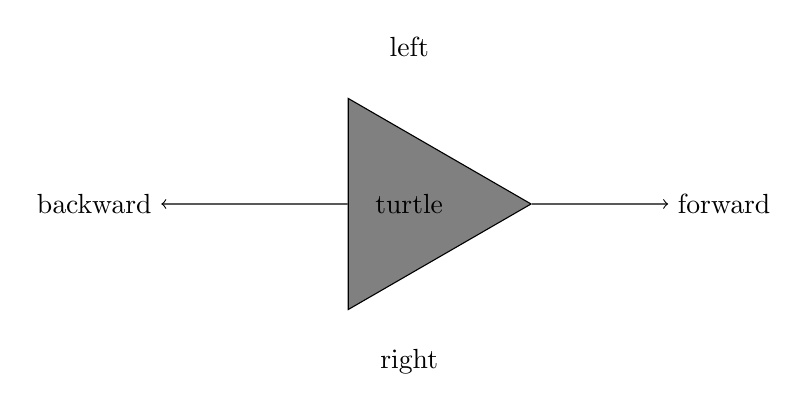
\begin{tikzpicture}

% nodes
\node (bk) at (4, 2) {backward};
\node[turtle] (tt) at (8, 2) {turtle};
\node (fd) at (12, 2) {forward};
\node (lt) at (8, 4) {left};
\node (rt) at (8, 0) {right};

% arrows
\draw[->] (tt) edge (bk);
\draw[->] (tt) edge (fd);

\end{tikzpicture}
\caption{绘图海龟的基本概念}
\end{figure}

许多分形构造或者铺嵌构造可以非常方便的通过一种支持裂解操作的 Logo 语言来实现。我们放宽原始 Logo 语言里的设定,
允许在画布上有多个海龟的存在,并且每个海龟单独维护自己的步长标准。于是,所谓的裂解是指一个操作,
它可以让一个海龟变成按照一定角度排布的多个海龟,同时新生成的海龟有新的步长设定。对于角度的排布,我们规定前进方向右侧转向是正的方向。

\begin{convention}
裂解采用如下的命令形式:
\begin{itemize}
\item 裂解[角度排布;步长设定]
\end{itemize}
\end{convention}

\newpage

\section{双曲几何}

结合几个材料的内容,本节我们介绍需要的双曲几何知识。

\subsection{反演变换}

给定平面 $\Pi$ 上一个圆 $\Phi$ 和圆外一点 $P$ ,可依次作直角三角形 $\bigtriangleup P N O$ 和 $\bigtriangleup N P^\prime O$ 。
如果圆 $\Phi$ 的半径是 $R$,不难推证:

\begin{equation} \label{e1}
|OP| \cdot |OP^\prime| = R^2
\end{equation}

\begin{definition}
\label{d1}
我们称映射 $\eta: P^\prime \mapsto P$ 为一个反演映射(inverse map),当且仅当它满足 \ref{e1} 式。
\end{definition}

\begin{figure}[ht]
\centering
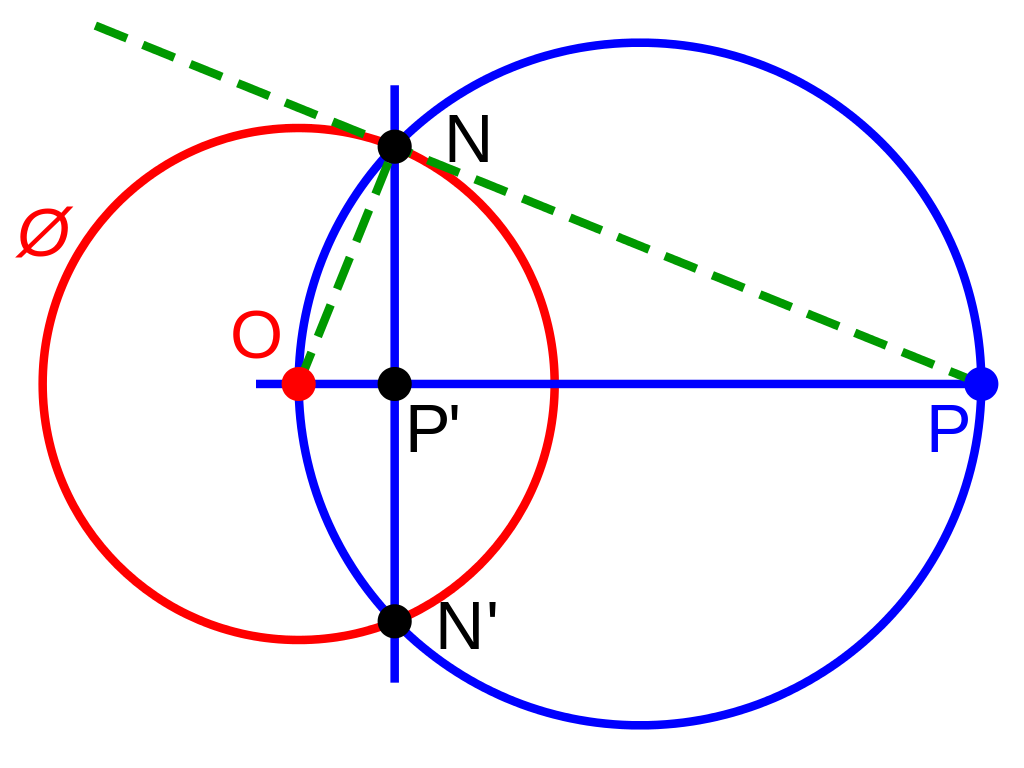
\includegraphics[width=3.5in]{images/inversion_in_circle.png}
\caption{反演变换下互逆的两个点}
\end{figure}

易见 $\eta$ 和 $\eta^-1$ 同为反演映射。映射 $\eta$在圆 $\Phi$ 的作用是恒等变换,点 $O$ 被映射到无穷远,
所以可以引入无穷远点 $\infty$ 使得 $\eta$ 在 $\Pi \cup \{\infty\}$ 上成为双射。

我们不加证明的引述下述命题:

\begin{itemize}
\item 反演变换 $\eta$ 是保角变换。
\item 平面 $\Pi$ 上任何圆或直线经反演变换 $\eta$ 后变换为圆或直线。
\item 平面 $\Pi$ 上任何与 $\Phi$ 正交的圆或直线经反演变换 $\eta$ 后变换为它们自身(不变子集)。
\end{itemize}

如果 $\Phi$ 是复平面的单位圆,我们有 $\eta$ 的复数表达:

$$\eta = \frac{1}{z}$$

\newpage

\subsection{庞加莱圆盘模型}

庞加莱圆盘是 2 维双曲几何 $H^2$ 的一种模型。我们考虑欧氏平面上的一个圆盘 $D$ ,我们在原来欧氏几何的基础上, 引入一种新的几何:
我们把边界 $\partial D$ 定义为无穷远,同时把垂直于 $\partial D$ 的圆弧(弧的两端都垂直于 $\partial D$)定义为新的几何上的直线。

\begin{figure}[ht]
\centering
\begin{tikzpicture}
    \draw (0, 0) node[inner sep=0] {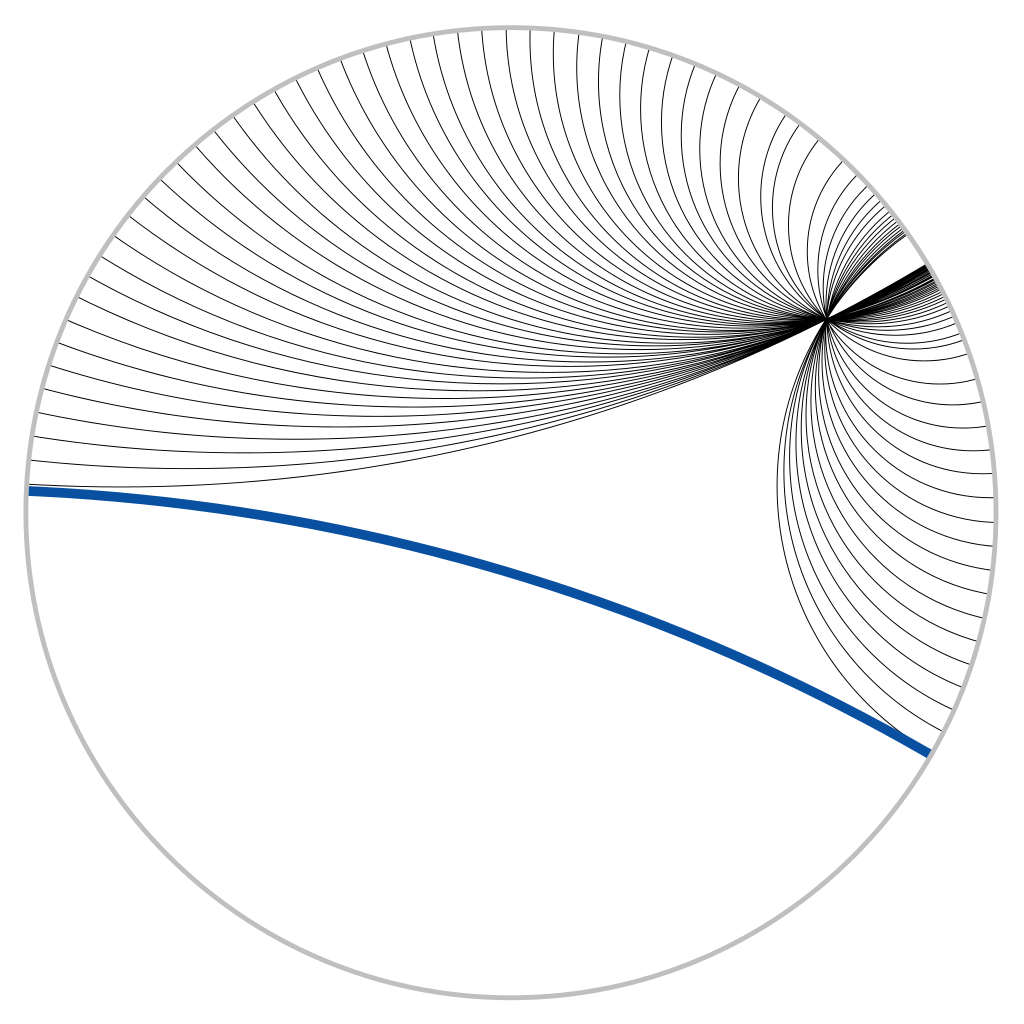
\includegraphics[width=3.5in]{images/hyperbolic_parallel.png}};
    \draw (+2.0, +1.0) node[inner sep=1pt] (p) {$P$};
    \draw (+0.0, -1.0) node[inner sep=1pt] (l) {$L$};
\end{tikzpicture}
\caption{过一点 P 与直线 L 平行的所有直线}
\end{figure}

在此基础上,我们可以引入新的几何上的直线间的平行关系。

新的几何上的直线间的垂直关系。

我们可以定义庞加莱圆盘上的距离。

\newpage

\subsection{角度、平行与垂直}

\subsection{理想点、理想三角形}

\subsection{极限圆}

\subsection{沿平行线推移}

\subsection{微分构造、距离构造、保角的构造?}

让我们回到基本的自己的问题,一步步踏实的走出来。

\newpage

\section{四阶无限边形铺嵌}

双曲平面上有许多非常有趣的铺嵌结构,这里我们展示一种称为四阶无限边形铺嵌的构造。
(调查清楚:四阶无限边形铺嵌需要一个特定的曲率?)

\begin{figure}[ht]
\centering
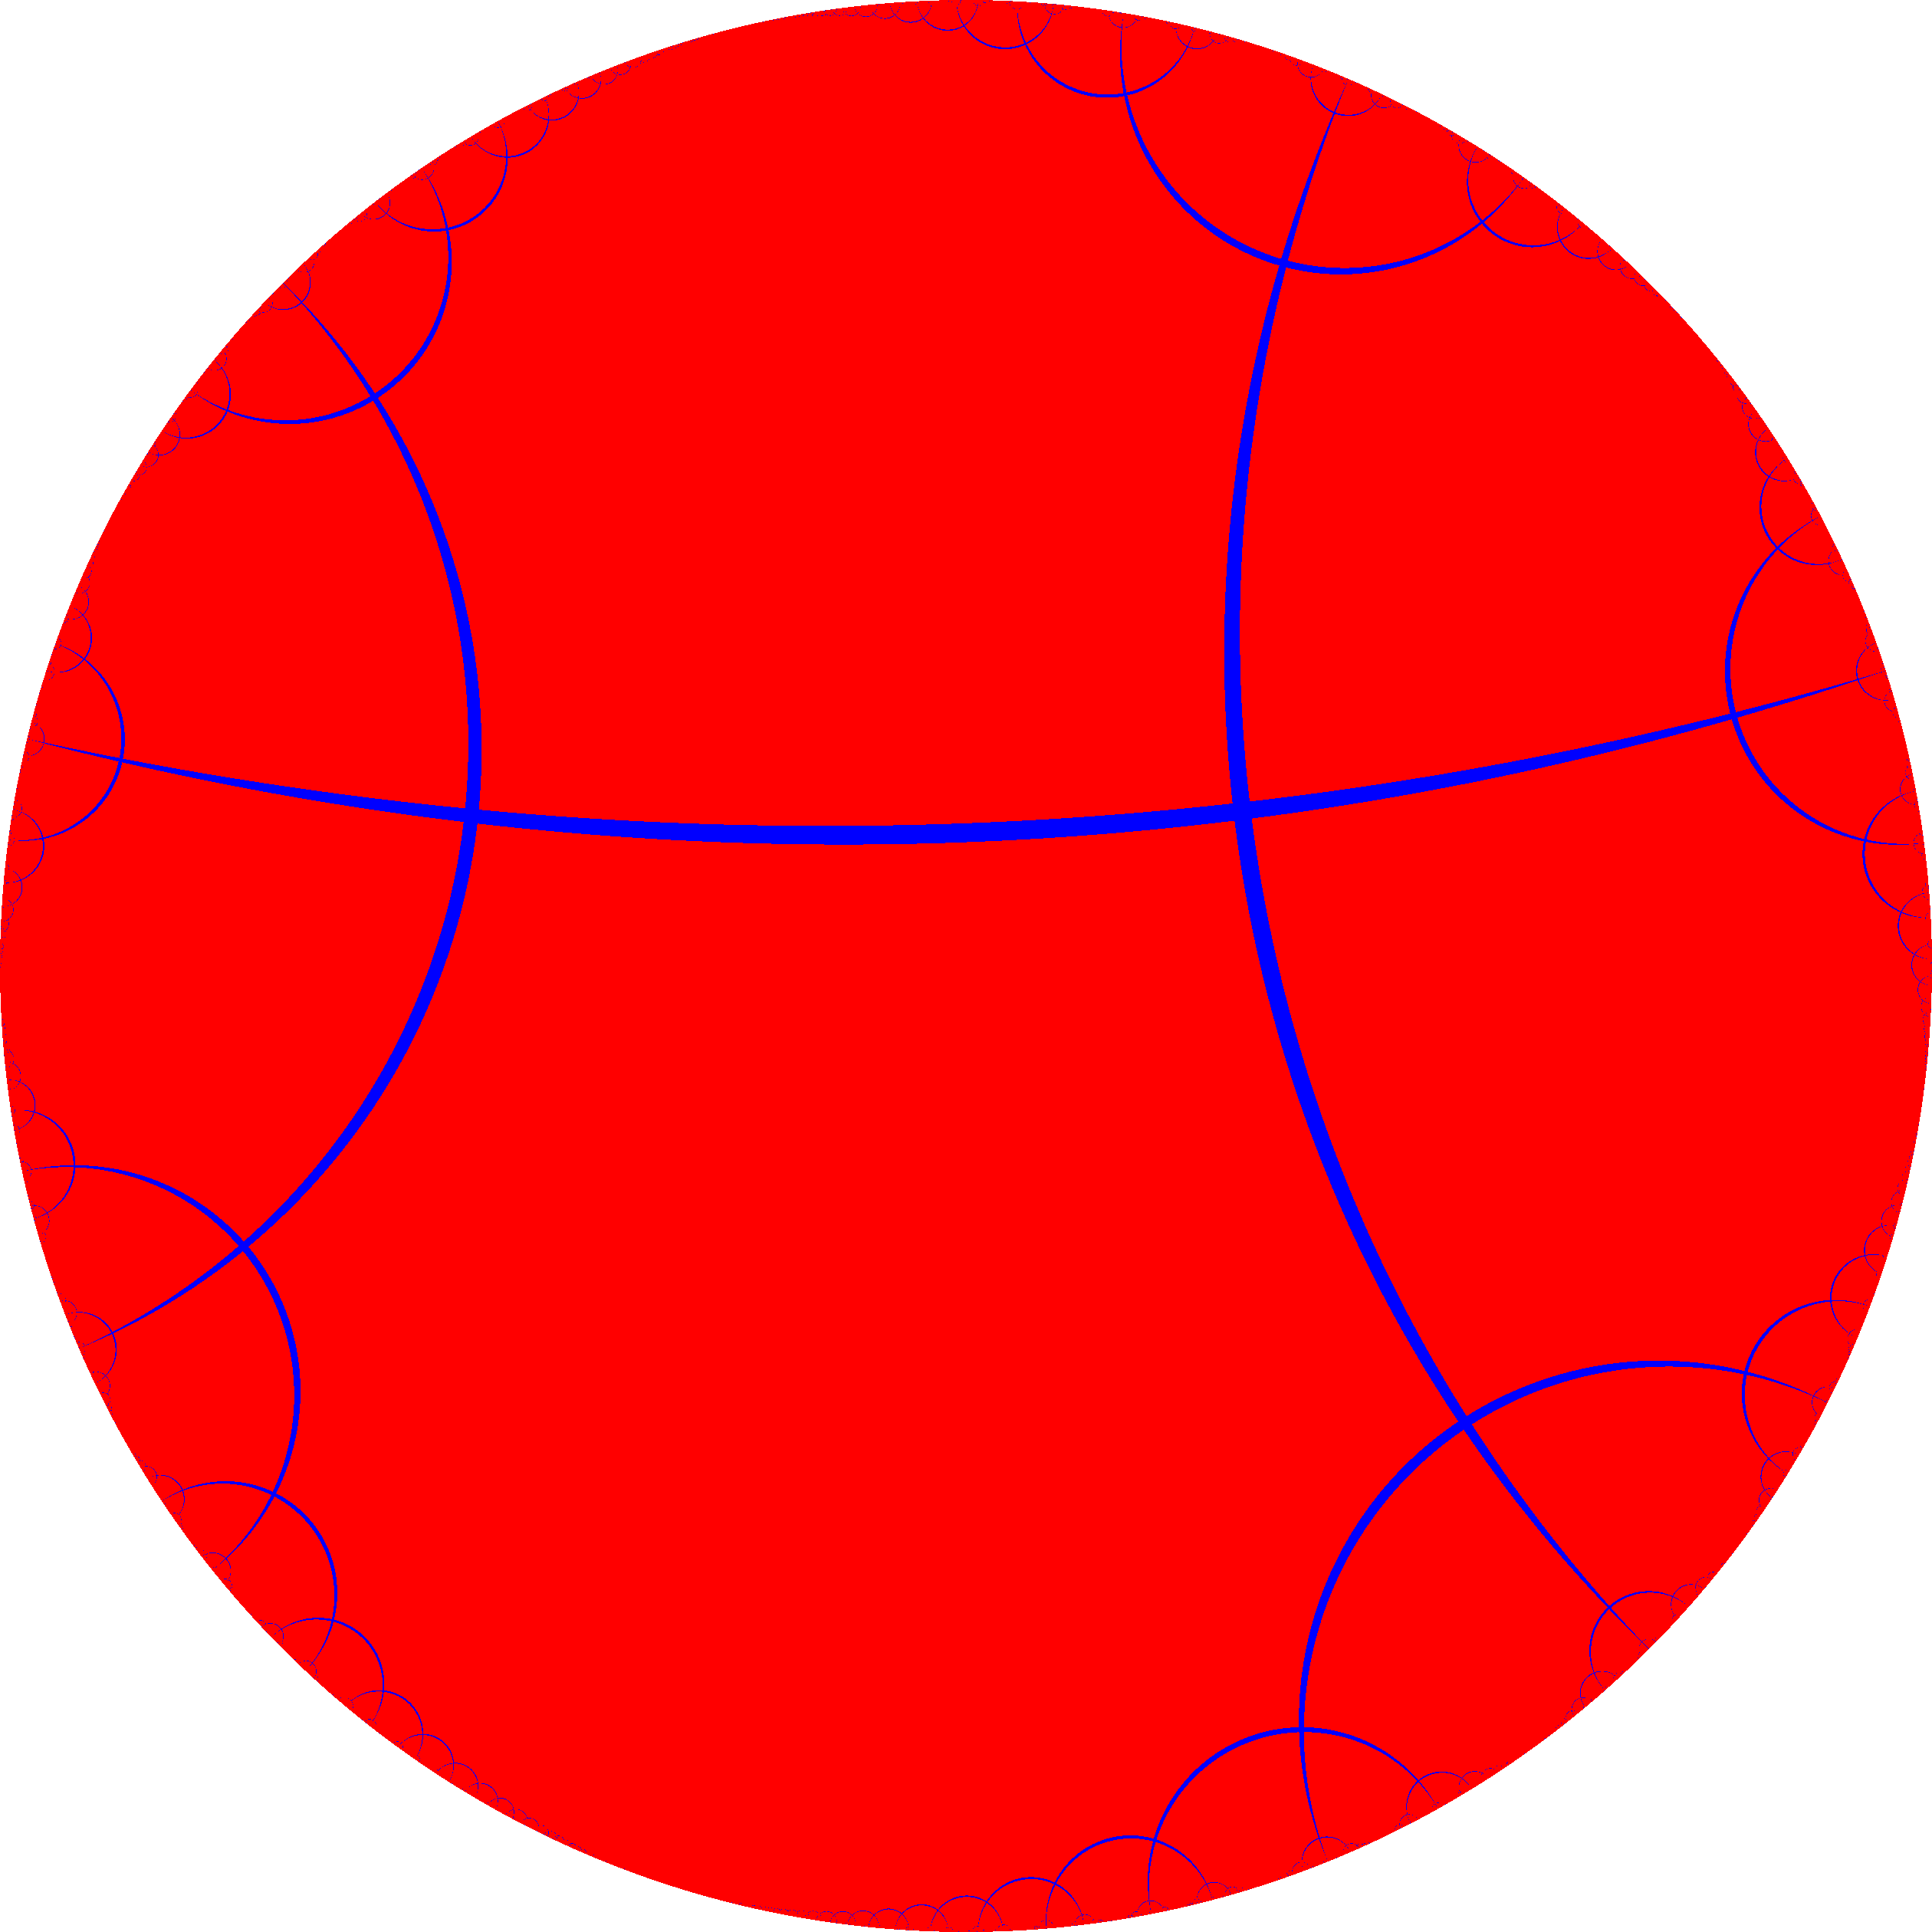
\includegraphics[width=3.5in]{images/H2_tiling_24i-1.png}
\caption{四阶无限边形铺嵌}
\end{figure}

这个铺嵌结构的构造程序如下

\begin{program}
四阶无限边形铺嵌的构造一
\begin{itemize}
\item 裂解[0, +90, +180, +270; 1]
\item 对所有的小海龟,反复无限次的执行下述命令
\begin{itemize}\item 前进一步 \item 裂解[-90, 0, +90; 1] \end{itemize}
\end{itemize}
\end{program}

如果注意到双曲平面是一个齐性空间,并且观察到在上述构造里,有些蓝色测地线之间彼此有交点,但这些交点彼此之间没有任何差别;
每一个交点都是两个测地线交汇出来的,都有四支分叉。利用对称性,我们容易理解:

\begin{proposition}
\label{A}
铺嵌结构上的两条测地线如果彼此之间相交,那么它们就是垂直的;否则这两条测地线就是平行的。
\end{proposition}

\begin{proposition}
\label{B}
对于任意一条铺嵌结构上的测地线,铺嵌结构上的其他测地线可以被归类到与之平行或垂直的两组之中。
\end{proposition}

\newpage

\subsection{铺嵌的其他方面}

\subsubsection{测地线 $\gamma$ 的六个无穷远点}

给到四阶无限边形铺嵌的上任意一条测地线 $\gamma$ 和其上的一点 $O$,非常直观的就会发现,
点 $O$ 旁边还有两条临近的测地线 $\alpha$ 和 $\beta$。三条测地线$\alpha$、$\beta$、$\gamma$分割出来六个区域,
对应有六个特殊的无穷远点。这六个特殊的无穷远点在庞加莱圆盘的视觉效果上有特殊的地方,
是铺嵌的树结构不同枝在无穷远处的视觉上的切触点,如下图所示:

\begin{figure}[ht]
\centering
\begin{tikzpicture}
    \draw (0, 0) node[inner sep=0] {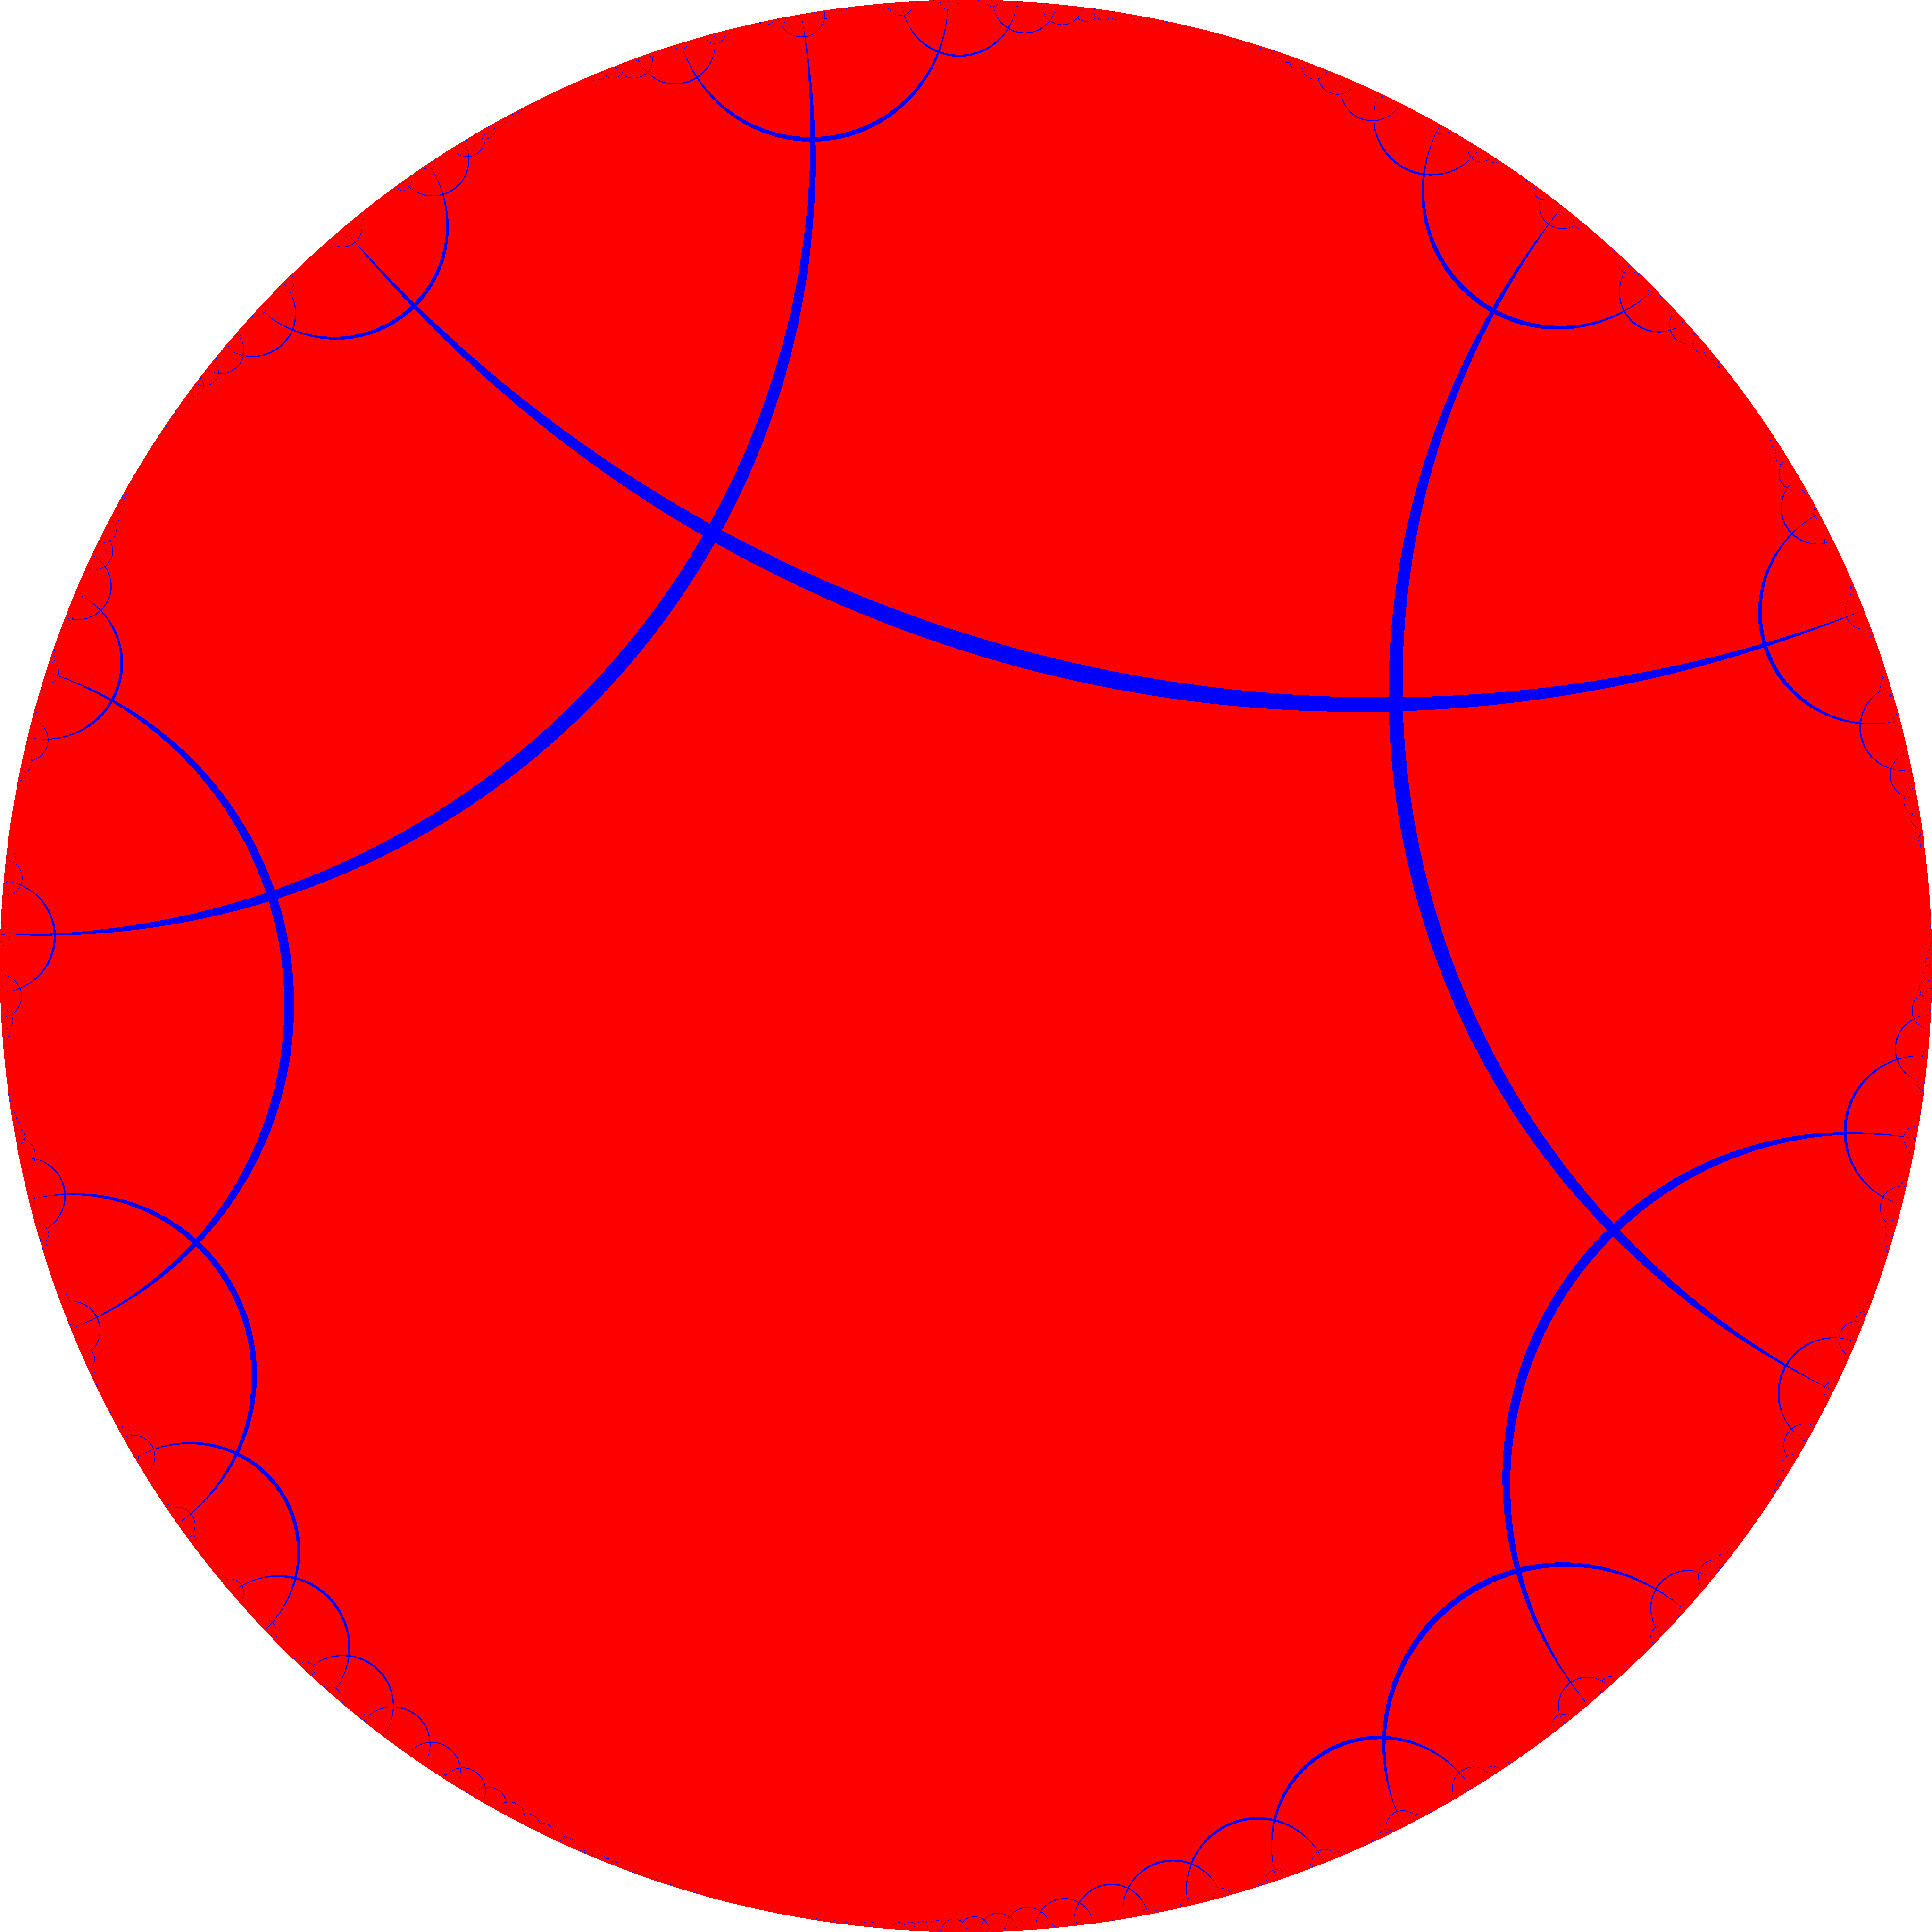
\includegraphics[width=6in]{images/t4096.png}};
    \draw (-1.80, +5.60) node[inner sep=1pt] (a) {$\alpha$};
    \draw (+3.20, +4.20) node[inner sep=1pt] (b) {$\beta$};
    \draw (+0.40, +1.60) node[inner sep=1pt] (g) {$\gamma$};
    \draw (+0.40, +2.70) node[inner sep=1pt, minimum size=0.2pt, above] (O) {$O$};
    \draw (+0.40, +2.45) node[circle, fill=black, inner sep=1pt, minimum size=0.5pt] (o) {};
    \draw (+1.89, +7.89) node[inner sep=1pt] (p_1) {$\infty_1$};
    \draw (-4.09, +7.04) node[inner sep=1pt] (p_2) {$\infty_2$};
    \draw (-7.23, +4.05) node[inner sep=1pt] (p_3) {$\infty_3$};
    \draw (-2.69, -7.89) node[inner sep=1pt] (p_4) {$\infty_4$};
    \draw (+8.38, +0.55) node[inner sep=1pt] (p_5) {$\infty_5$};
    \draw (+6.63, +4.75) node[inner sep=1pt] (p_6) {$\infty_6$};

\end{tikzpicture}
\caption{六个特殊的无穷远点}
\end{figure}

\newpage

\subsubsection{引入镜面映射}

\begin{figure}[ht]
\centering
\begin{tikzpicture}
    \draw (0, 0) node[inner sep=0] {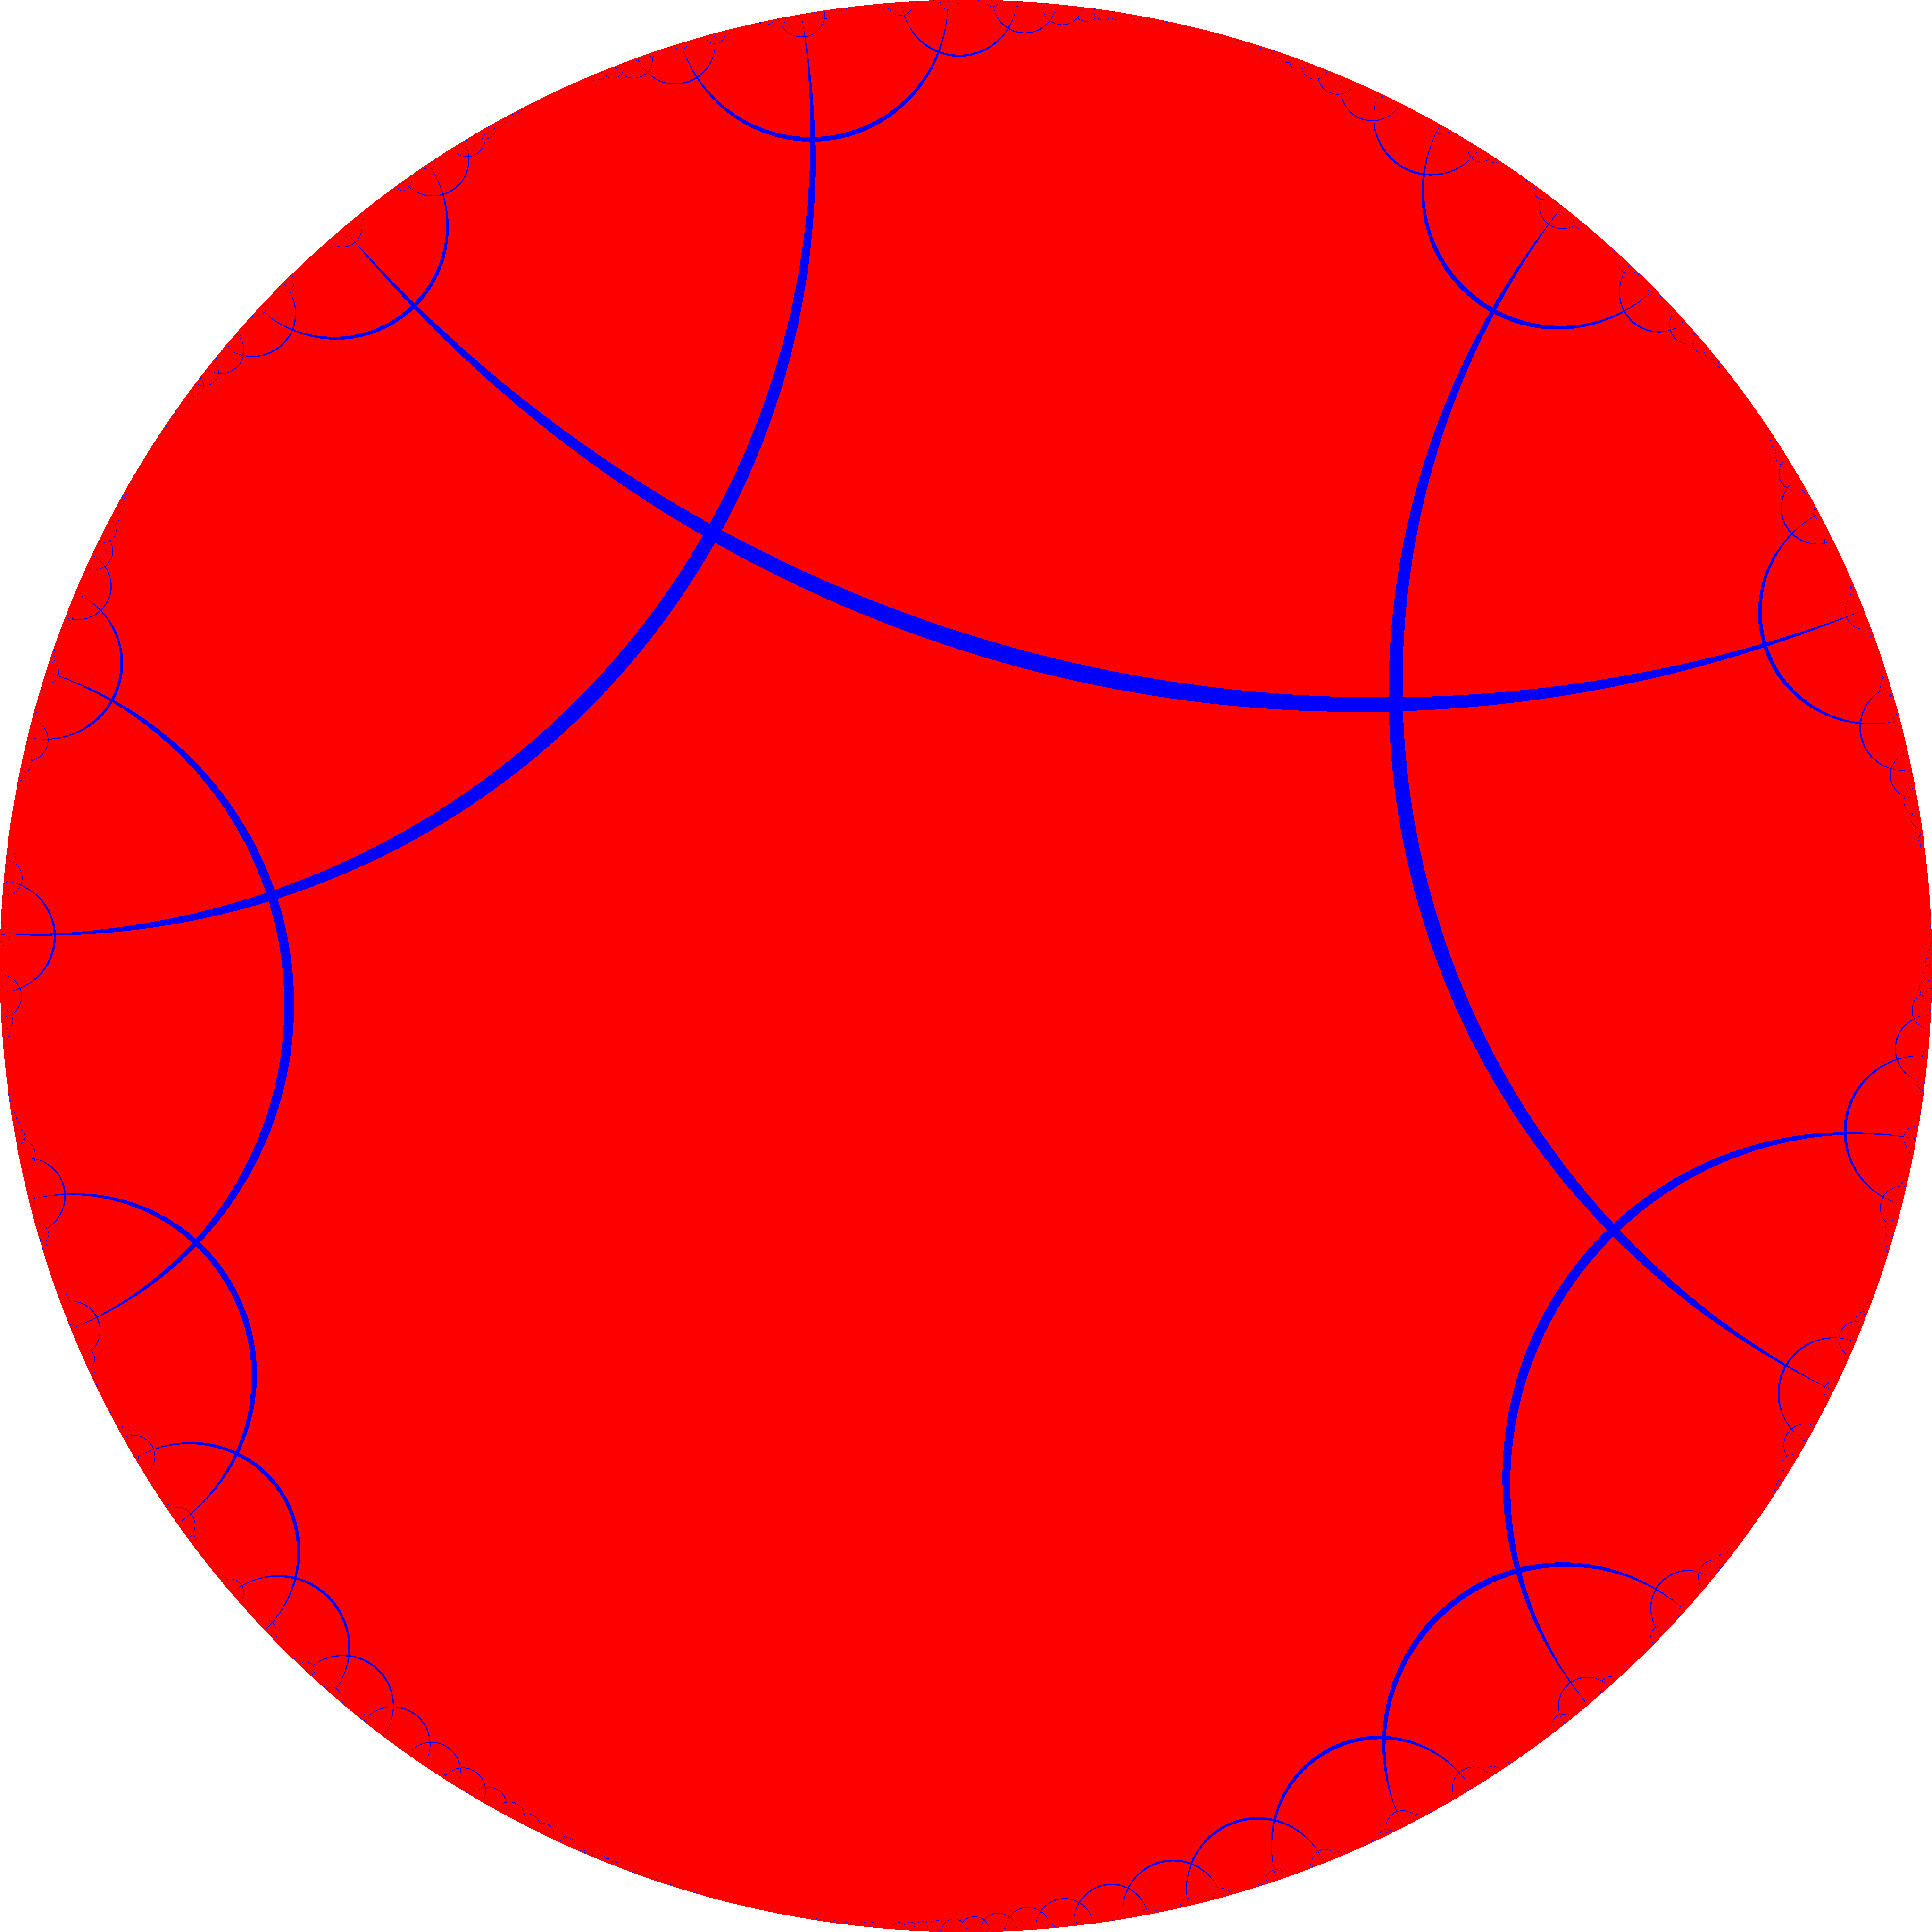
\includegraphics[width=6in]{images/t4096.png}};
    \draw (-4.00, +4.20) node[inner sep=1pt] (g) {$\gamma$};
    \draw (+1.80, +5.20) node[inner sep=1pt] (g_0) {$g_0$};
    \draw (+1.89, +7.89) node[inner sep=1pt] (p_1) {$\infty_1$};
    \draw (-4.09, +7.04) node[inner sep=1pt] (p_2) {$\infty_2$};
    \draw (-7.23, +4.05) node[inner sep=1pt] (p_3) {$\infty_3$};
    \draw (-2.69, -7.89) node[inner sep=1pt] (p_4) {$\infty_4$};
    \draw (+8.38, +0.55) node[inner sep=1pt] (p_5) {$\infty_5$};
    \draw (+6.63, +4.75) node[inner sep=1pt] (p_6) {$\infty_6$};

    \draw [black, dotted, line width=1mm]
          (-1.89, -7.39) node[inner sep=1pt] (p_pinf) {}
       -- (+1.89, +7.39) node[inner sep=1pt] (p_ninf) {};
\end{tikzpicture}
\caption{镜面映射的轴}
\end{figure}

连接 $\infty_1$ 和 $\infty_4$ 得到镜面映射的轴$g_0$。$g_0$是测地线。

\newpage

\subsubsection{沿测地线 $\gamma$ 推移镜面结构}

如上小节所述,首先我们有测地线 $\gamma$ 和 测地线 $g_0$,在它们旁边是测地线 $g_{-1}$ 和 测地线 $g_1$。
我们连接 $\infty_2$ 和 $\infty_3$ 得到测地线$g_{-2}$,连接 $\infty_5$ 和 $\infty_6$ 得到测地线$g_{2}$。

\begin{figure}[ht]
\centering
\begin{tikzpicture}
    \draw (0, 0) node[inner sep=0] {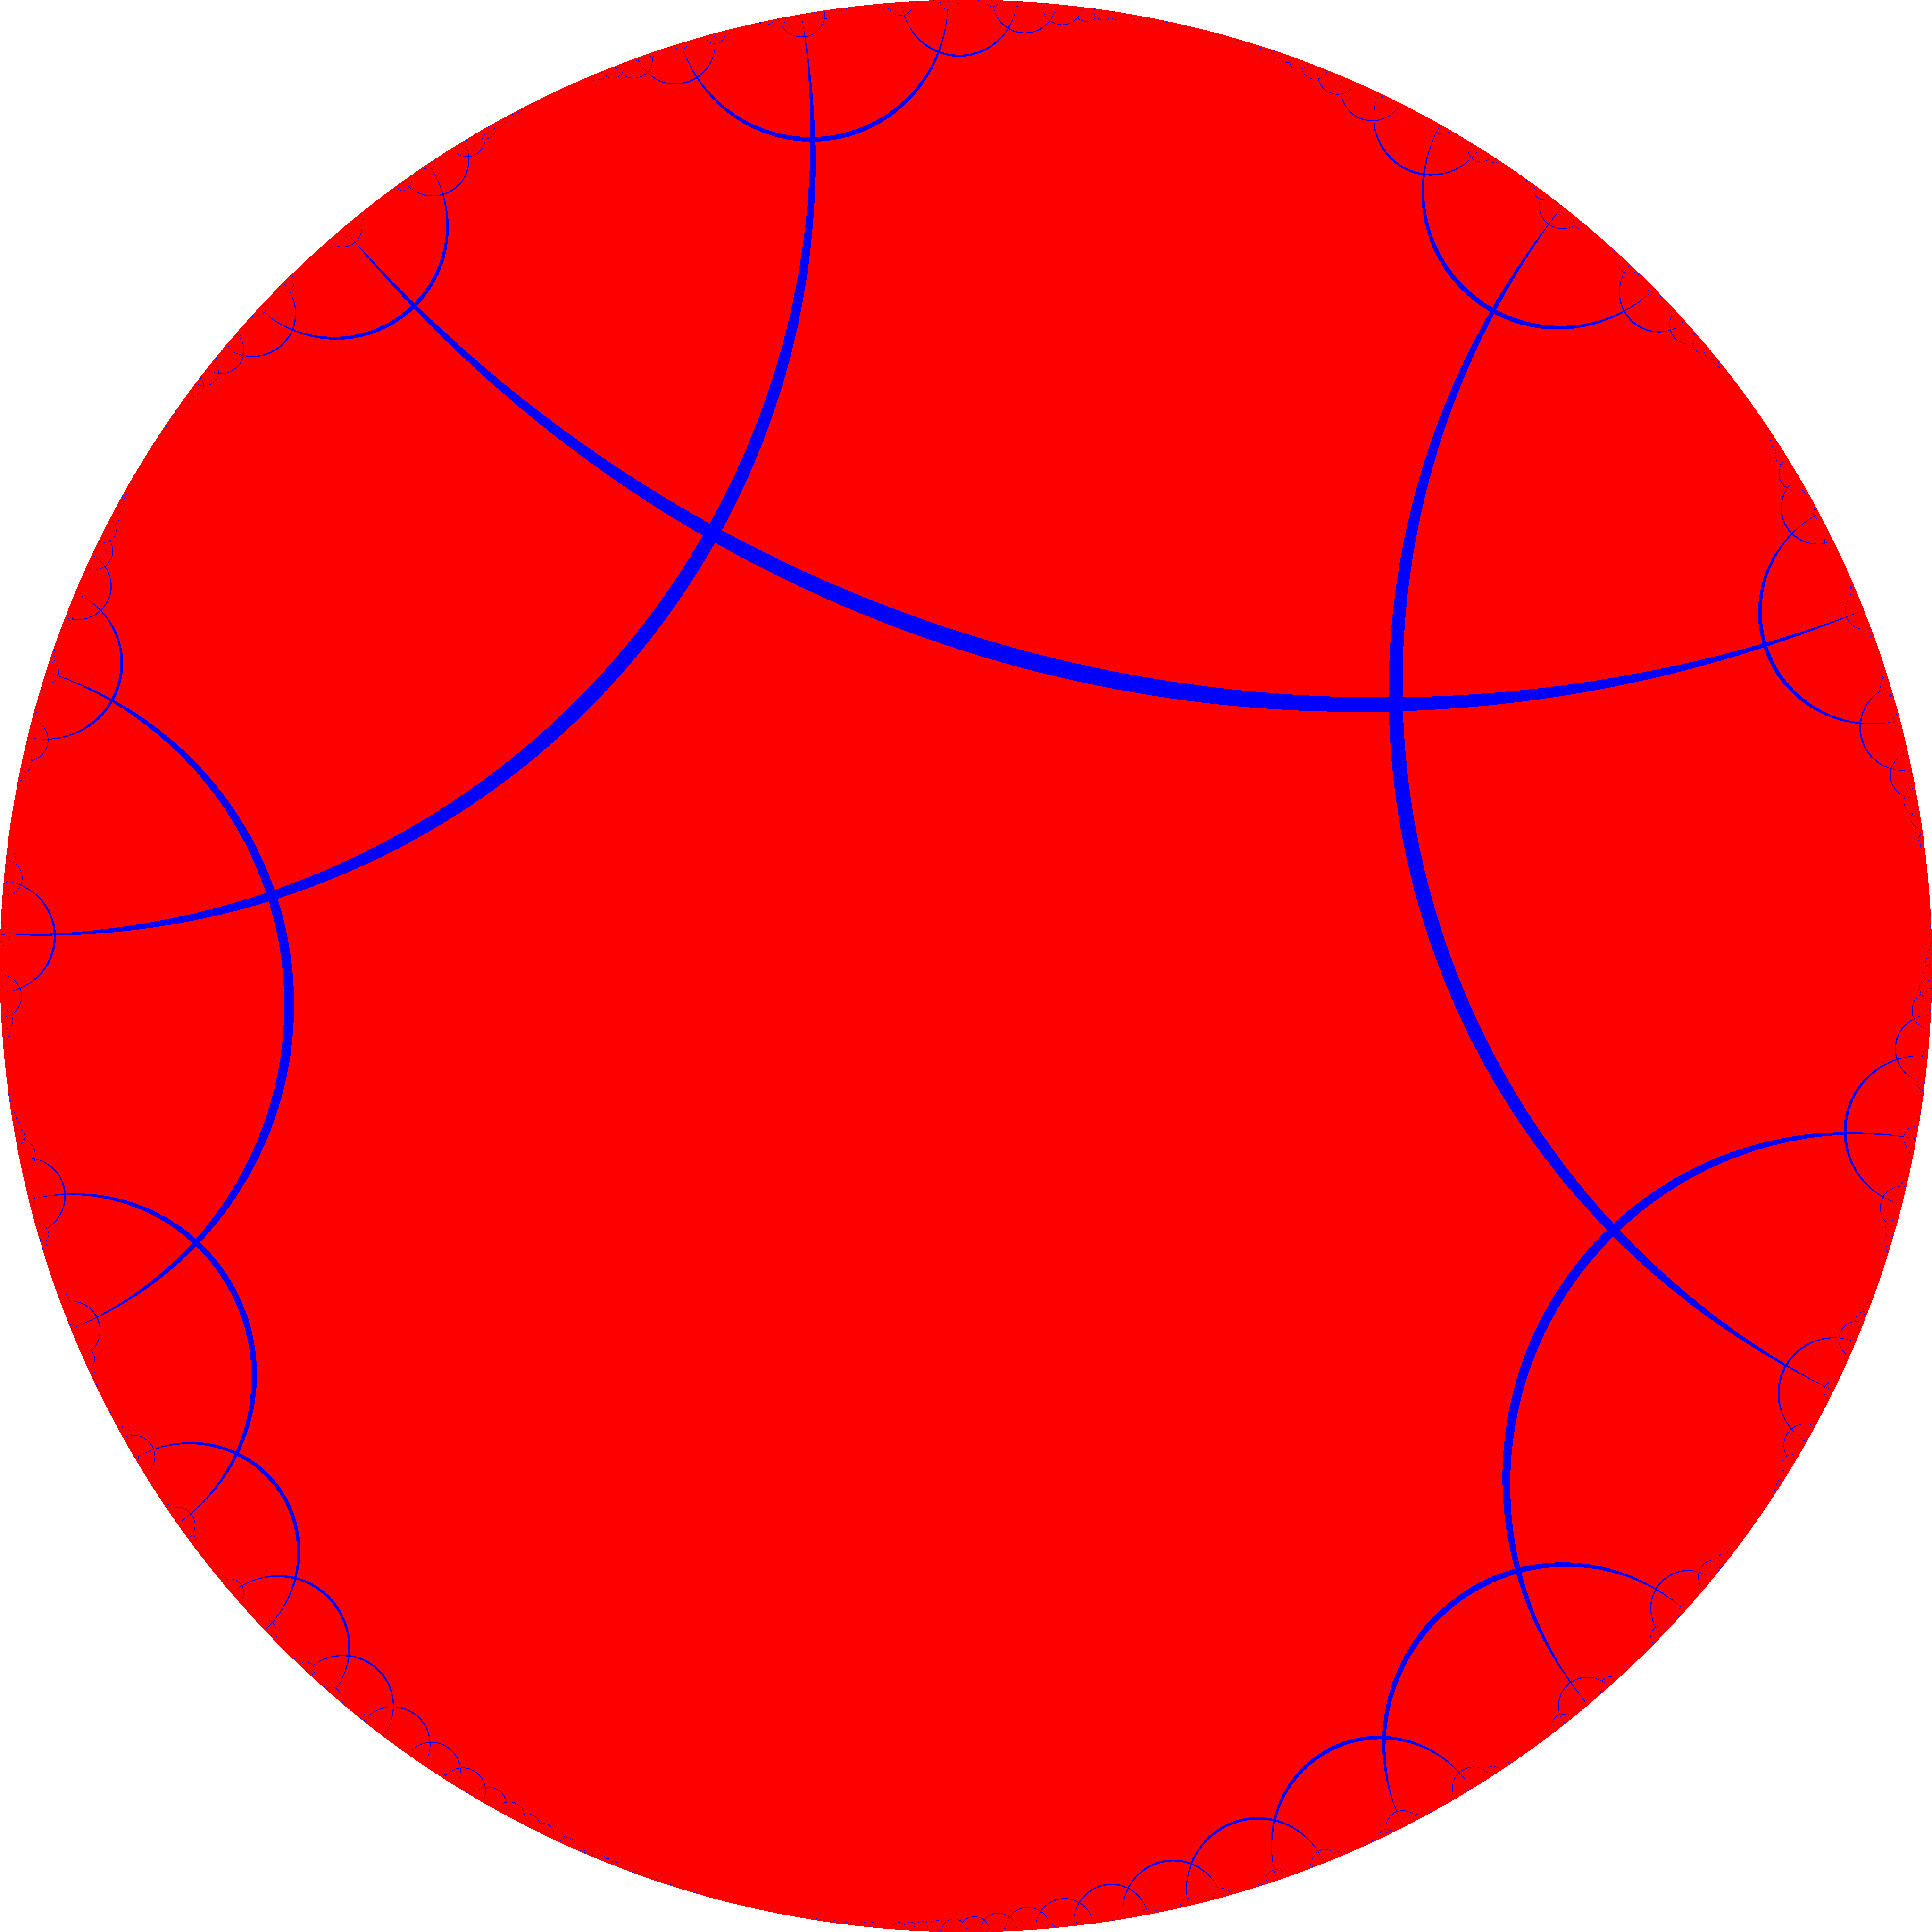
\includegraphics[width=6in]{images/t4096.png}};
    \draw (+1.50, +1.70) node[inner sep=1pt] (g) {$\gamma$};
    \draw (-2.50, +4.50) node[inner sep=1pt] (g_n2) {$g_{-2}$};
    \draw (-1.80, +5.00) node[inner sep=1pt] (g_n1) {$g_{-1}$};
    \draw (+1.80, +5.20) node[inner sep=1pt] (g_0) {$g_0$};
    \draw (+4.00, +4.00) node[inner sep=1pt] (g_p1) {$g_1$};
    \draw (+5.00, +2.80) node[inner sep=1pt] (g_p2) {$g_2$};
    \draw (+1.89, +7.89) node[inner sep=1pt] (p_1) {$\infty_1$};
    \draw (-4.09, +7.04) node[inner sep=1pt] (p_2) {$\infty_2$};
    \draw (-7.23, +4.05) node[inner sep=1pt] (p_3) {$\infty_3$};
    \draw (-2.69, -7.89) node[inner sep=1pt] (p_4) {$\infty_4$};
    \draw (+8.38, +0.55) node[inner sep=1pt] (p_5) {$\infty_5$};
    \draw (+6.63, +4.75) node[inner sep=1pt] (p_6) {$\infty_6$};

    % geodesic 0 %
    \draw [black, dotted, line width=1mm]
          (-1.89, -7.39) node[inner sep=1pt] (p_pinf) {}
       -- (+1.89, +7.39) node[inner sep=1pt] (p_ninf) {};

    % geodesic 1 %
    \draw [black, dotted, line width=1mm]
          (-3.29, 6.84) arc (205.0:58.7:-2.20);

    % line 0 %
    \draw [green, dotted, thick]
          (-3.29, 6.84) arc (240:271.7:18.00);

    % geodesic 1 %
    \draw [black, dotted, line width=1mm]
          (7.58, 0.55) arc (265.0:135.7:2.25);

   % line 1 %
    \draw [green, dotted, thick]
          (-6.43, 4.05) arc (240:271.7:26.50);

\end{tikzpicture}
\caption{沿测地线 $\gamma$ 推移镜面结构}
\end{figure}

想象我们有一台摄像机在庞加莱圆盘对应的双曲平面 $H_2$ 里移动,摄像机拍摄出来的广角画面就是我们看到的庞加莱圆盘。
如果我们沿测地线 $\gamma$ 推移摄像机,看到的广角画面会怎么样呢?
\begin{itemize}
    \item 左移摄像机会看到:$g_0$ 会连续变到 $g_1$、$g_2$ 的位置上。
    \item 右移摄像机会看到:$g_0$ 会连续变到 $g_{-1}$、$g_{-2}$ 的位置上。
\end{itemize}

\newpage

\subsection{铺嵌的对偶}

%\begin{figure} \centering
%\begin{tikzpicture}[
%        every node/.style={anchor=south west,inner sep=0pt},
%        x=1mm, y=1mm,
%      ]
%     \node (fig1) at (0, 0)
%       {\includegraphics[width=6in]{i24.png}};
%     \node (fig2) at (0, 0)
%       {\includegraphics[width=6in]{i42.png}};
%\end{tikzpicture}
%\caption{对偶}
%\end{figure}

两个对偶为什么不是几何上完全对称?是计算误差还是其他原因。

\newpage

\subsection{H-树}

H-树是如下图所示的分形构造。四阶无限边形铺嵌按照一定规则剪枝,拓扑上可以得到H-树。

\begin{figure}[ht]
\centering
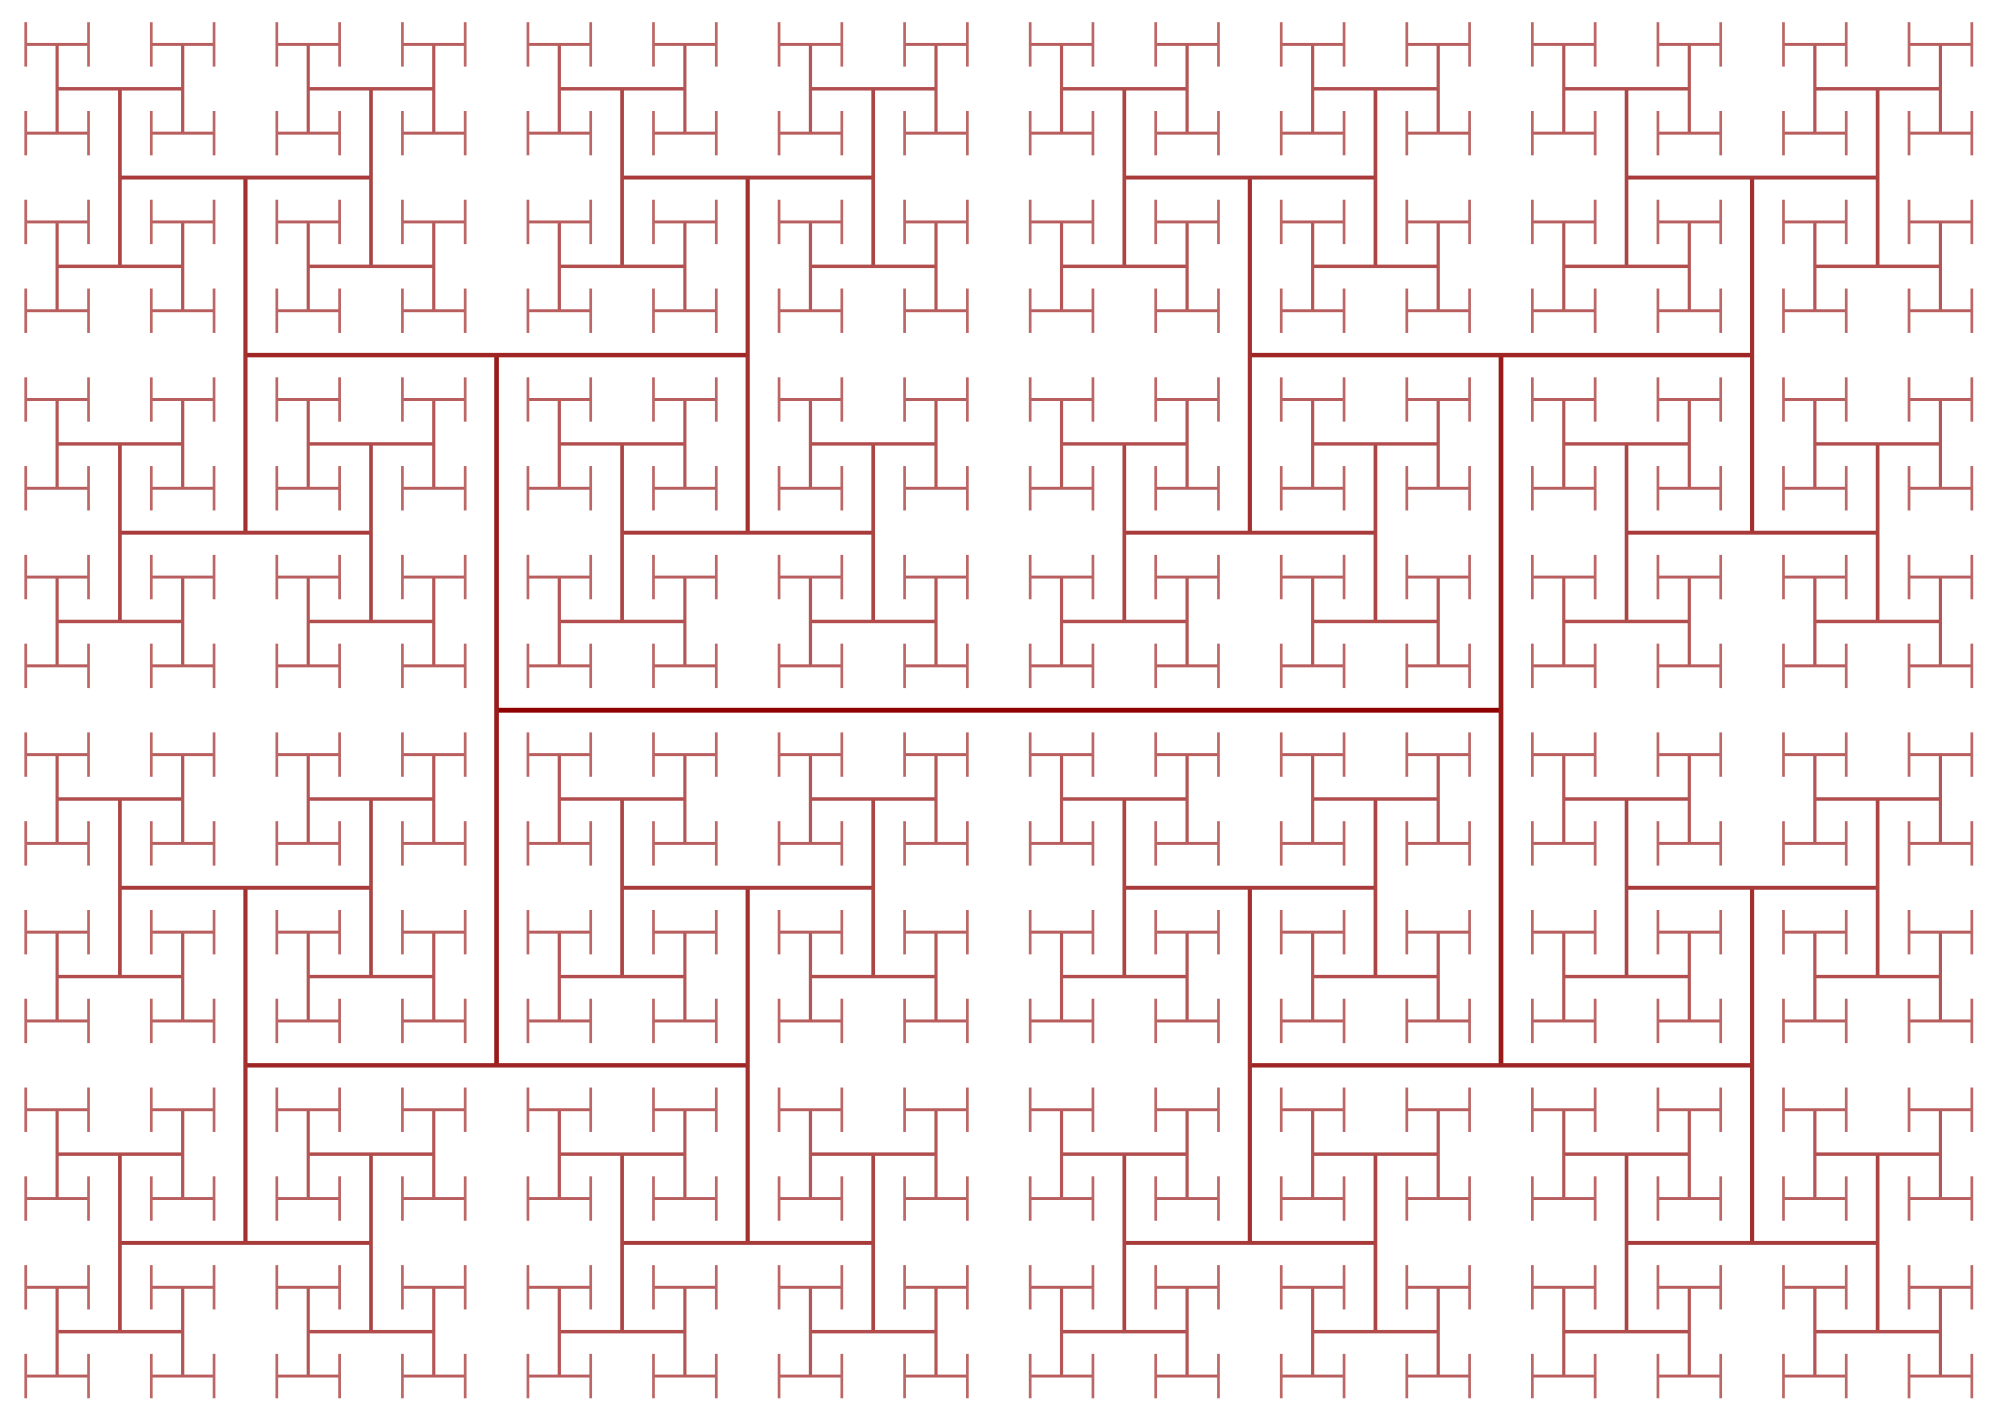
\includegraphics[width=3.5in]{images/2000px-H_tree.png}
\caption{H-树}
\end{figure}

H-树的具体构造程序如下

\begin{program}
H-树的构造
\begin{itemize}
\item 对所有的小海龟,反复无限次的执行下述命令
\begin{itemize}\item 前进一步 \item 裂解[-90, +90; $\sqrt{2} / 2$] \end{itemize}
\end{itemize}
\end{program}

\newpage

\section{希尔伯特曲线}

希尔伯特曲线是另外一种分形构造,可以理解成是围绕着 $\Pi$ 的某种一笔画展开。希尔伯特曲线的相邻各段是彼此垂直的,但长度并不相同。

\begin{figure}[ht]
\centering
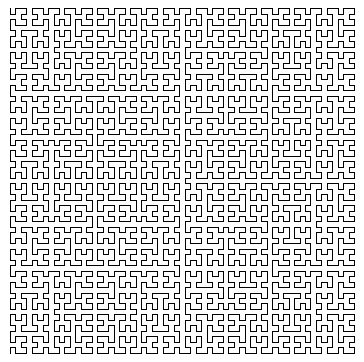
\includegraphics[width=3.5in]{images/hilbert.png}
\caption{希尔伯特曲线}
\end{figure}

下面我们把希尔伯特曲线这种空间填充方式和一种称为超现实数的特殊构造联系在一起。

\newpage

\section{超现实数}

超现实数按照生成树的先序遍历是严格从小到大的。超现实数是一种序和代数的结构,有非常强大的序关系。

\begin{figure}[ht]
\centering
\begin{tikzpicture}
    \draw (0, 0) node[inner sep=0] {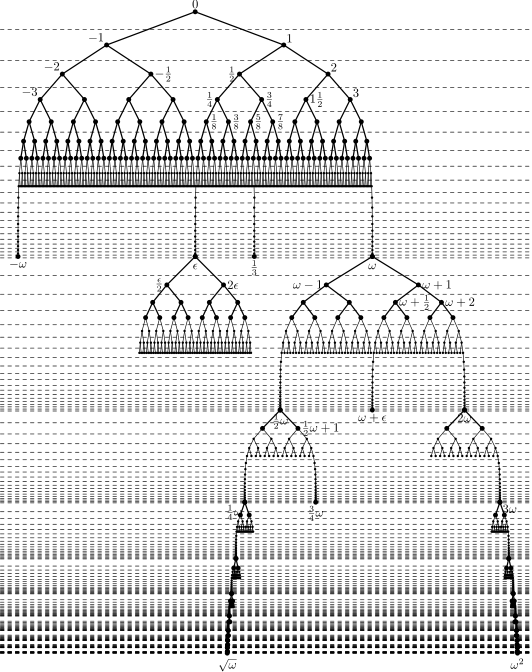
\includegraphics[width=3in]{images/surreal.png}};
\end{tikzpicture}
\caption{超现实数的生成树}
\end{figure}

我们把超现实数的有理数前面的部分写出来。

\begin{figure}[ht]
\centering
\begin{tikzpicture}
    \draw (0, 0) node[inner sep=0] {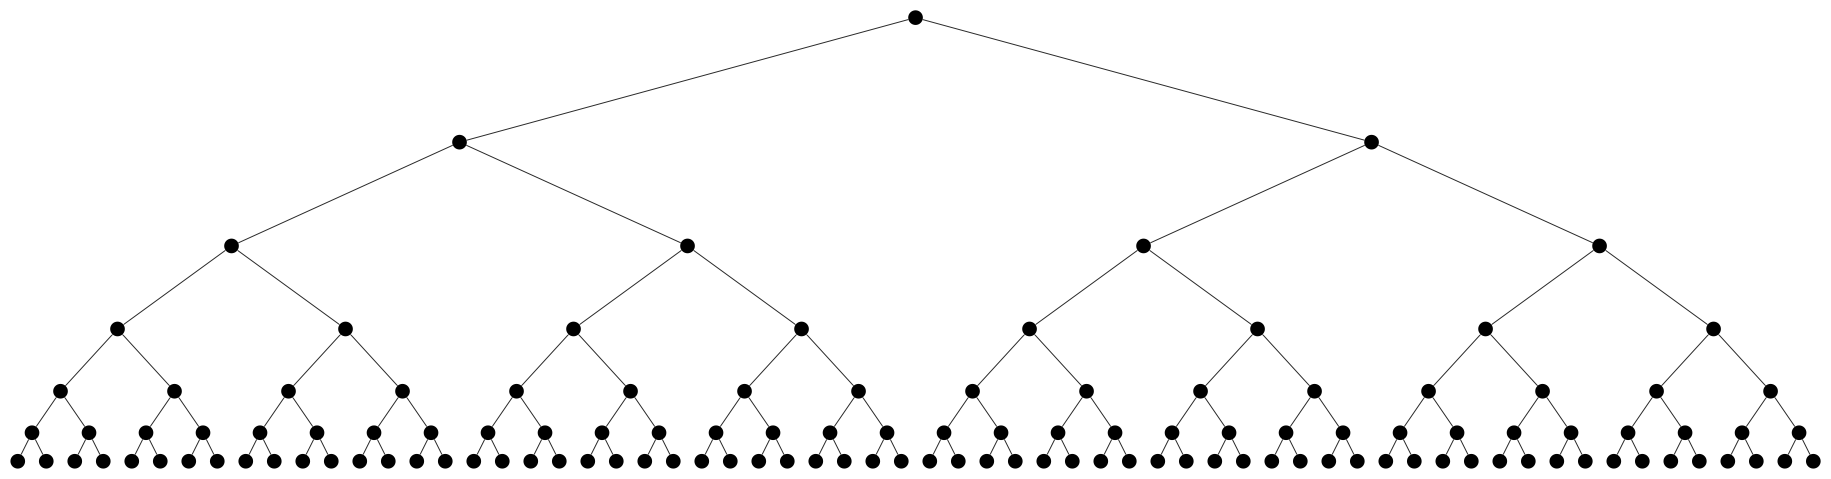
\includegraphics[width=6in]{images/tree.png}};
\end{tikzpicture}
\caption{超现实数的有理数部分}
\end{figure}

\newpage

\subsection{超现实数局部几何化}

结合希尔伯特曲线重新理解超现实数。

\newpage

\section{加乘树 $\mathfrak{K}$}

一个基本的想法是,我们能否探索计算的过程,而不仅仅限于计算的结果。

\subsection{加乘树的引入}

\begin{figure}[ht]
\centering
\begin{tikzpicture}
    \draw (0, 0) node[inner sep=0] {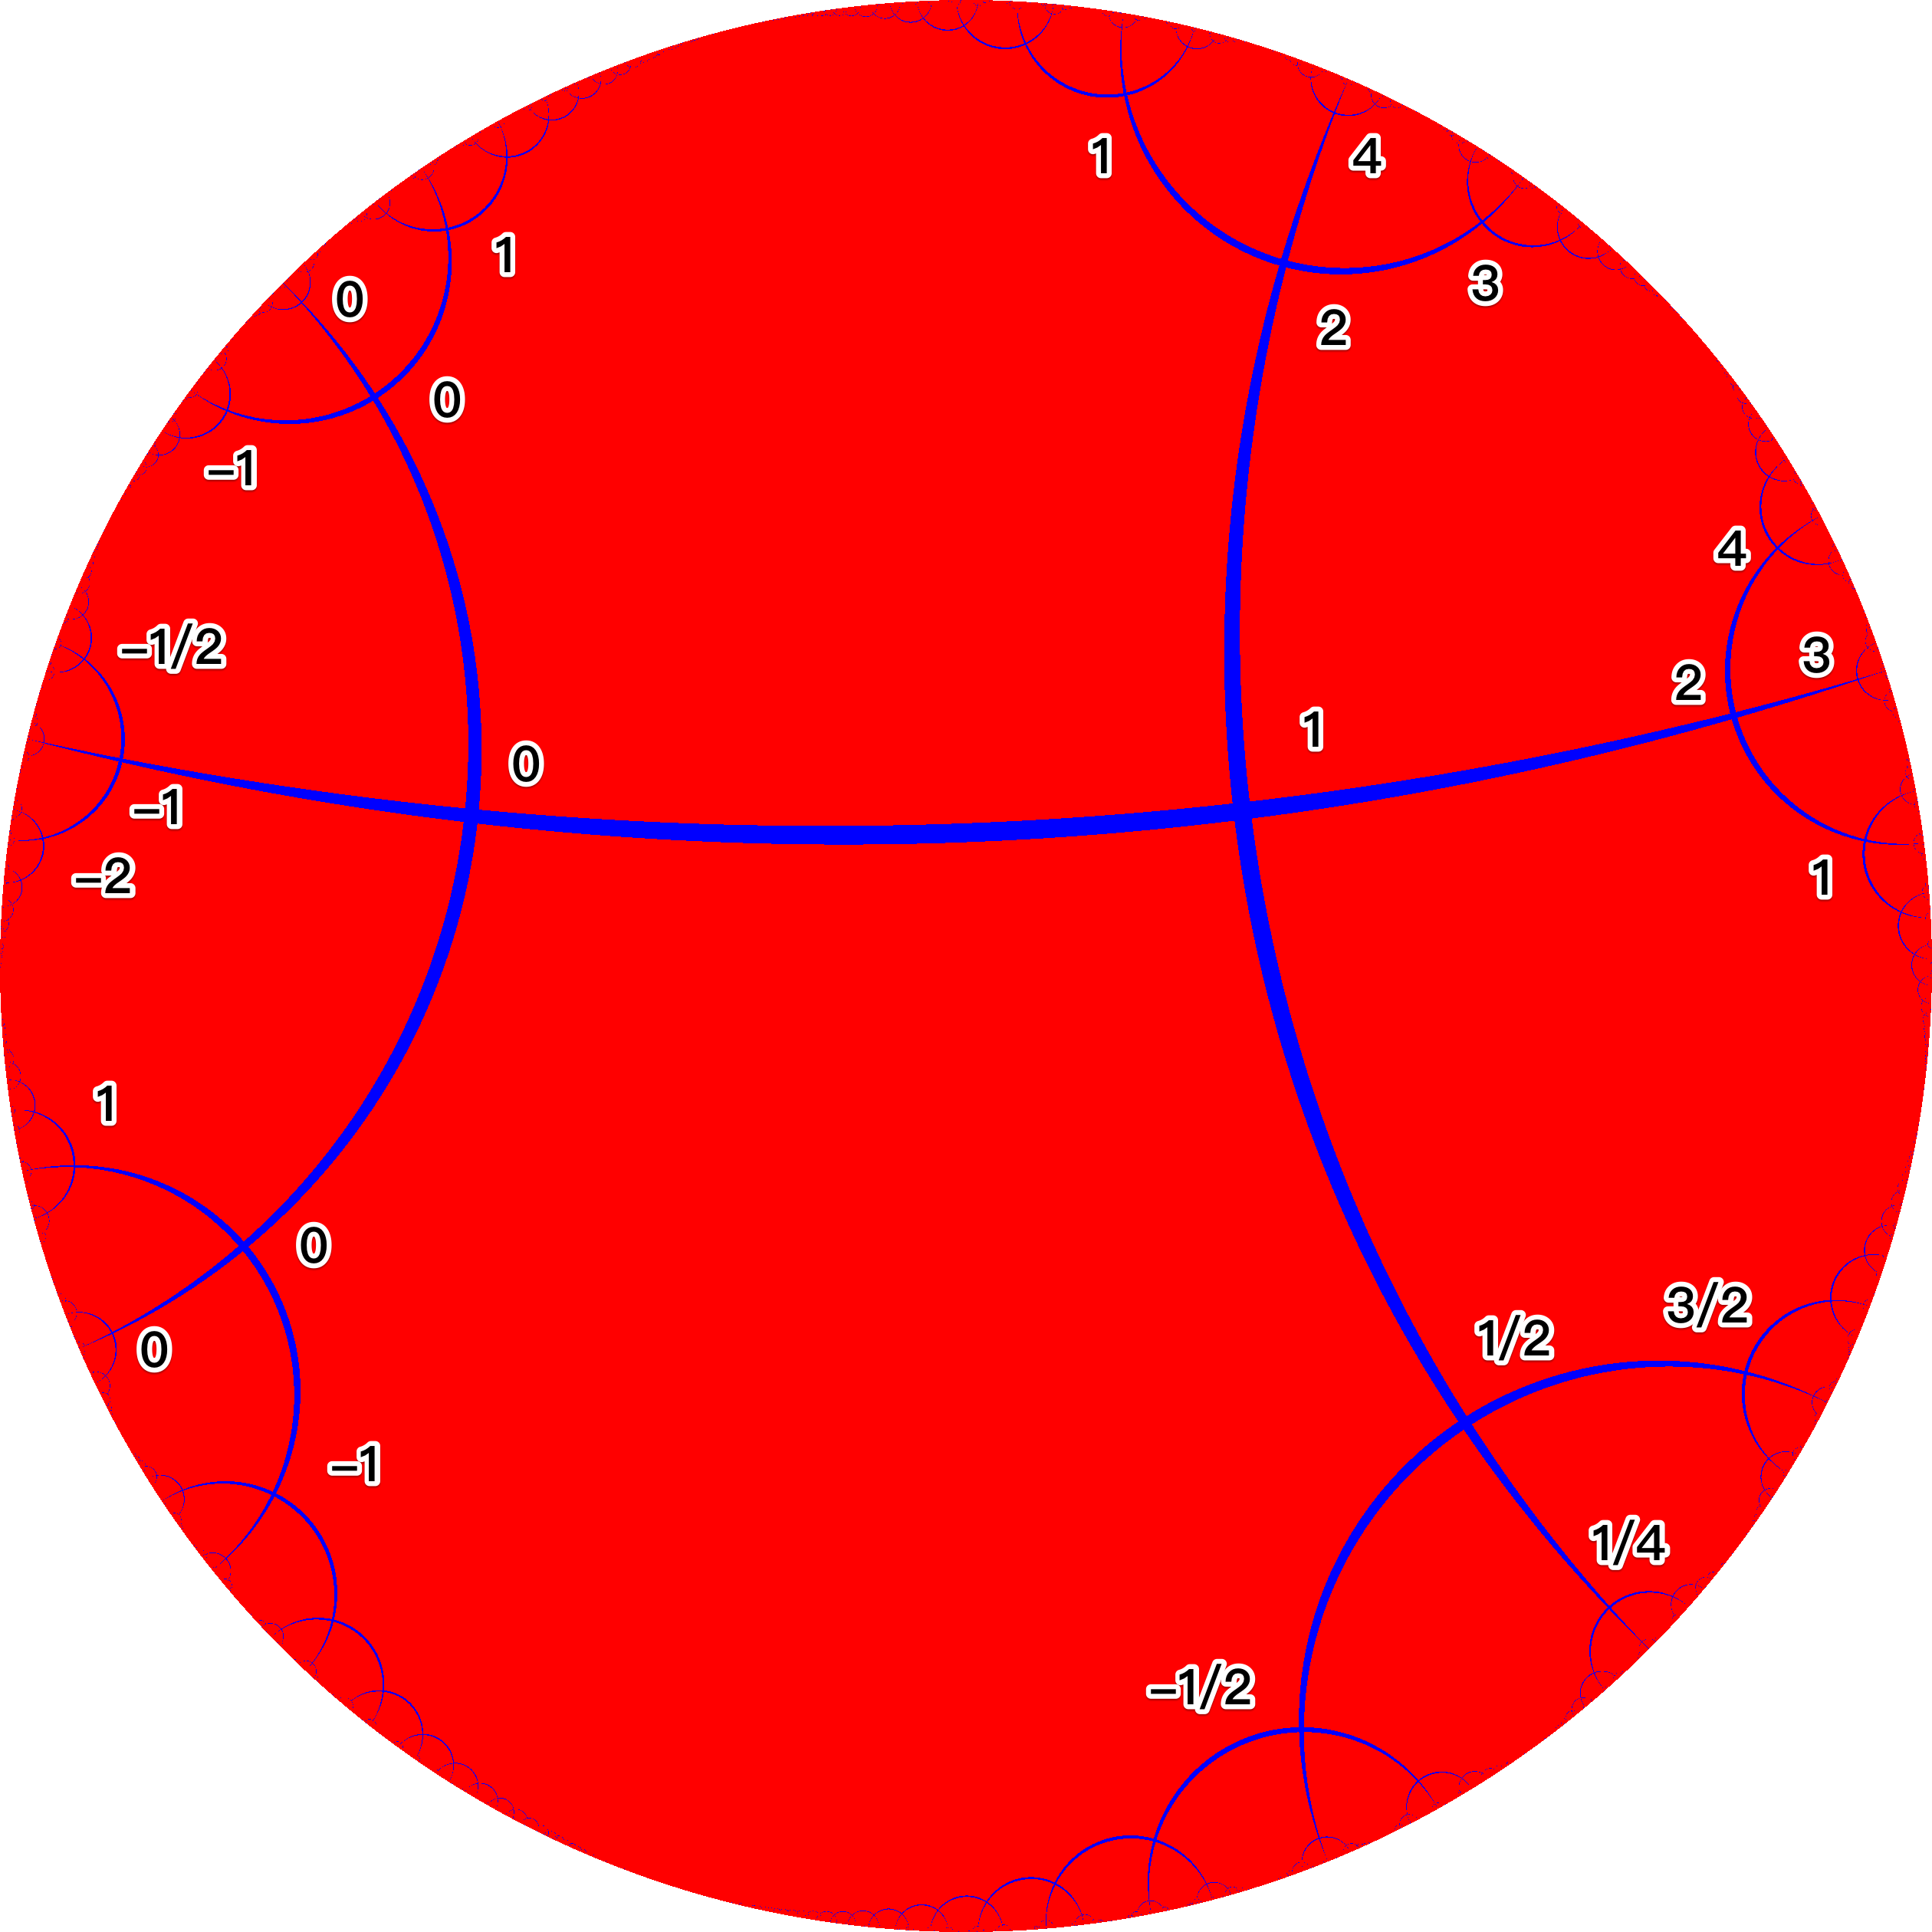
\includegraphics[width=6in]{images/H2_tiling_with_assign_1.png}};
\end{tikzpicture}
\caption{加乘树带来的赋值}
\end{figure}

\subsection{计算过程的几何化}


\subsection{观察角度}

因为加乘树像万花筒(Kaleidoscope)一样可以看到非常多的数学对象,我们把加乘树的系统用记号 $\mathfrak{K}$ 代表。

\newpage

\section{嵌入超现实数的想法}

超现实数的生成树具有高度的规律性,我们猜测超现实数的生成树可以嵌入到加乘树里面,而且每个树枝都是一条测地线。

目前能看到的

推证一:加乘树、自相似性 $\Rightarrow$ 局部希尔伯特填充

推证二:局部希尔伯特填充、超现实数生成树 $\Rightarrow$ 全局的希尔伯特填充

推证三:全局的希尔伯特填充 $\Rightarrow$ 黎曼共形映射定理

嵌入超现实数的想法需要和无穷远点的垂直联系起来,注定是个不平凡的东西。

\subsection{嵌入$0$}

\begin{figure}[ht]
\centering
\begin{tikzpicture}
    \draw (0, 0) node[inner sep=0] {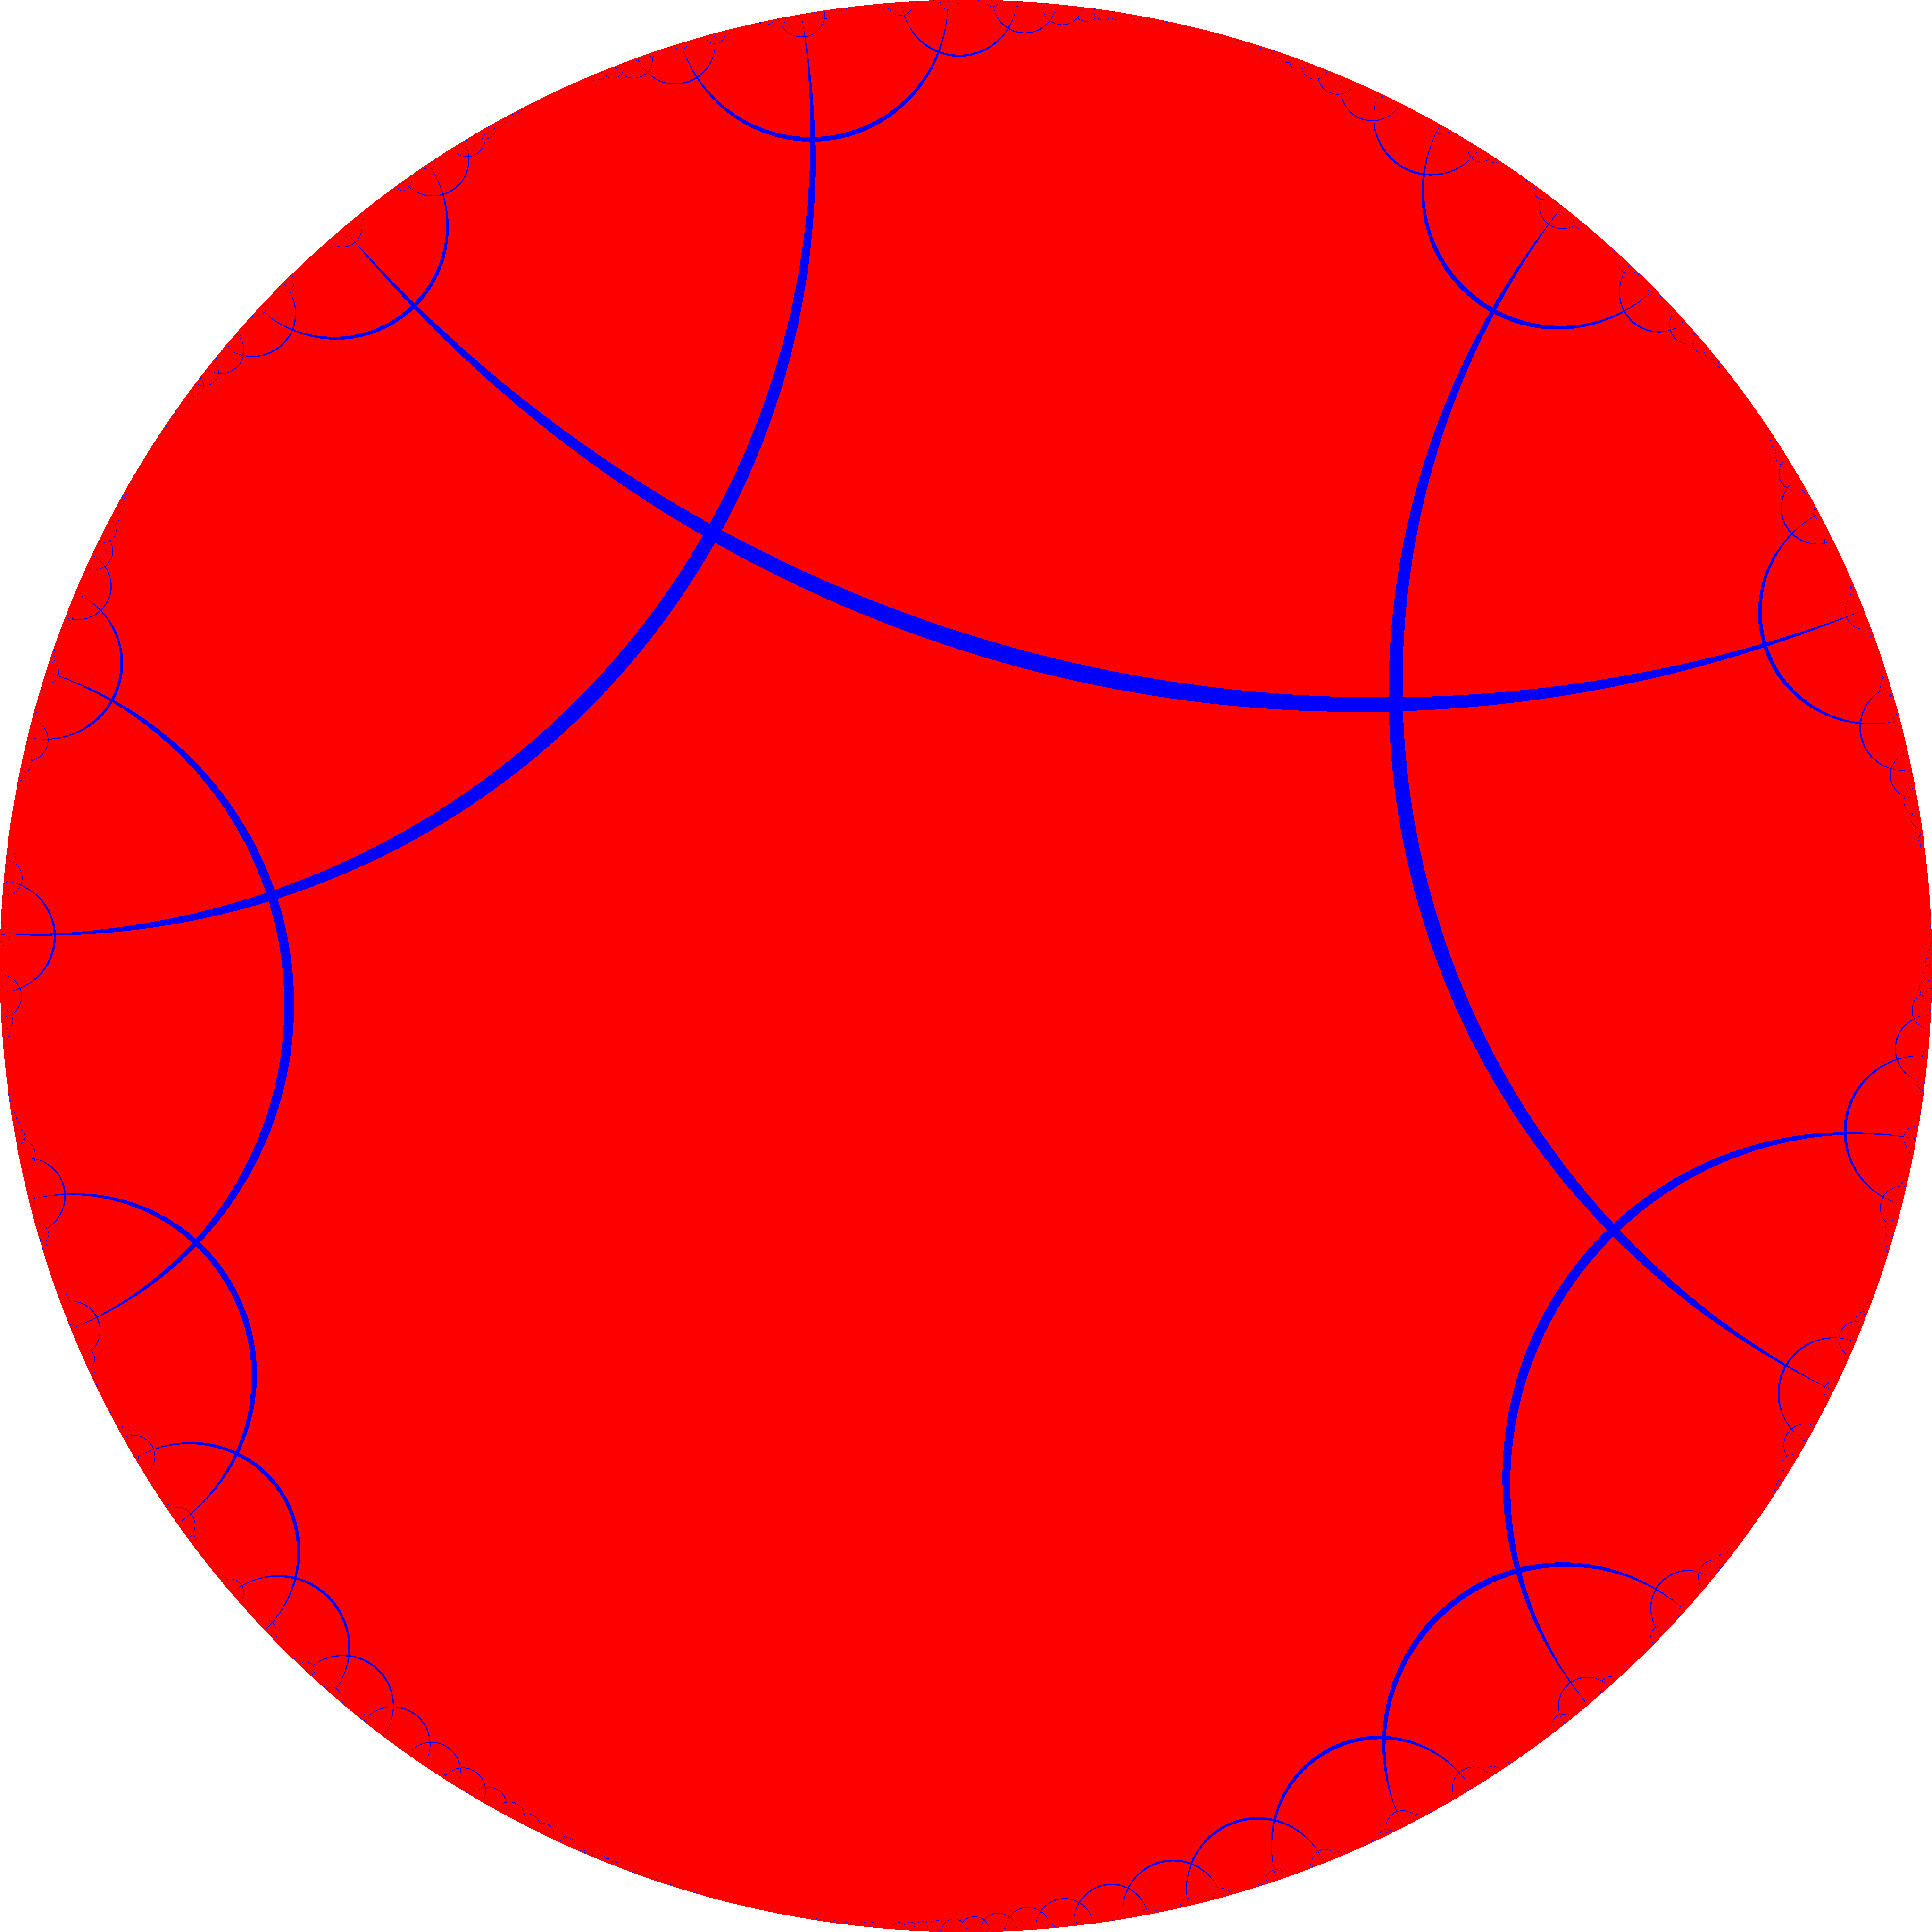
\includegraphics[width=6in]{images/t4096.png}};
    \draw (-1.35, -3.50) node[inner sep=1pt] (p_z) {0};

    % geodesic 0 %
    \draw [black, dotted, line width=0.3mm]
          (-1.89, -7.39) node[inner sep=1pt] (p_pinf) {}
       -- (+1.89, +7.39) node[inner sep=1pt] (p_ninf) {};

    \draw (-0.9, +6.2) node {$-1$};
    \draw (-1.9, +2.9) node {$-\frac{1}{2}$};
    \draw (-5.0, +0.3) node {$-\frac{1}{4}$};
    \draw (-7.0, +0.0) node {$-\frac{1}{8}$};

    \draw (+3.7, +4.9) node {$+1$};
    \draw (+3.1, +1.7) node {$+\frac{1}{2}$};
    \draw (+5.2, -2.5) node {$+\frac{1}{4}$};
\end{tikzpicture}
\caption{嵌入$0$ 线}
\end{figure}

在 $0$ 的附近不难找到一条加线由 $-\frac{1}{2}$ 和 $\frac{1}{2}$ 标定。
如上图,我们可以引入一条零线 $0$,该零线和原来的加线相交于中点 $0$。

\newpage

\subsection{嵌入$n$}

由 $-\frac{1}{2}$ 和 $\frac{1}{2}$ 标定的加线上原本分布着 $\frac{2n + 1}{2}$ 这些点。
但显然,随着上小节零线和零点的引入,$n$ 这些点也自然的出现在这条加线上。

\begin{figure}[ht]
\centering
\begin{tikzpicture}
    \draw (0, 0) node[inner sep=0] {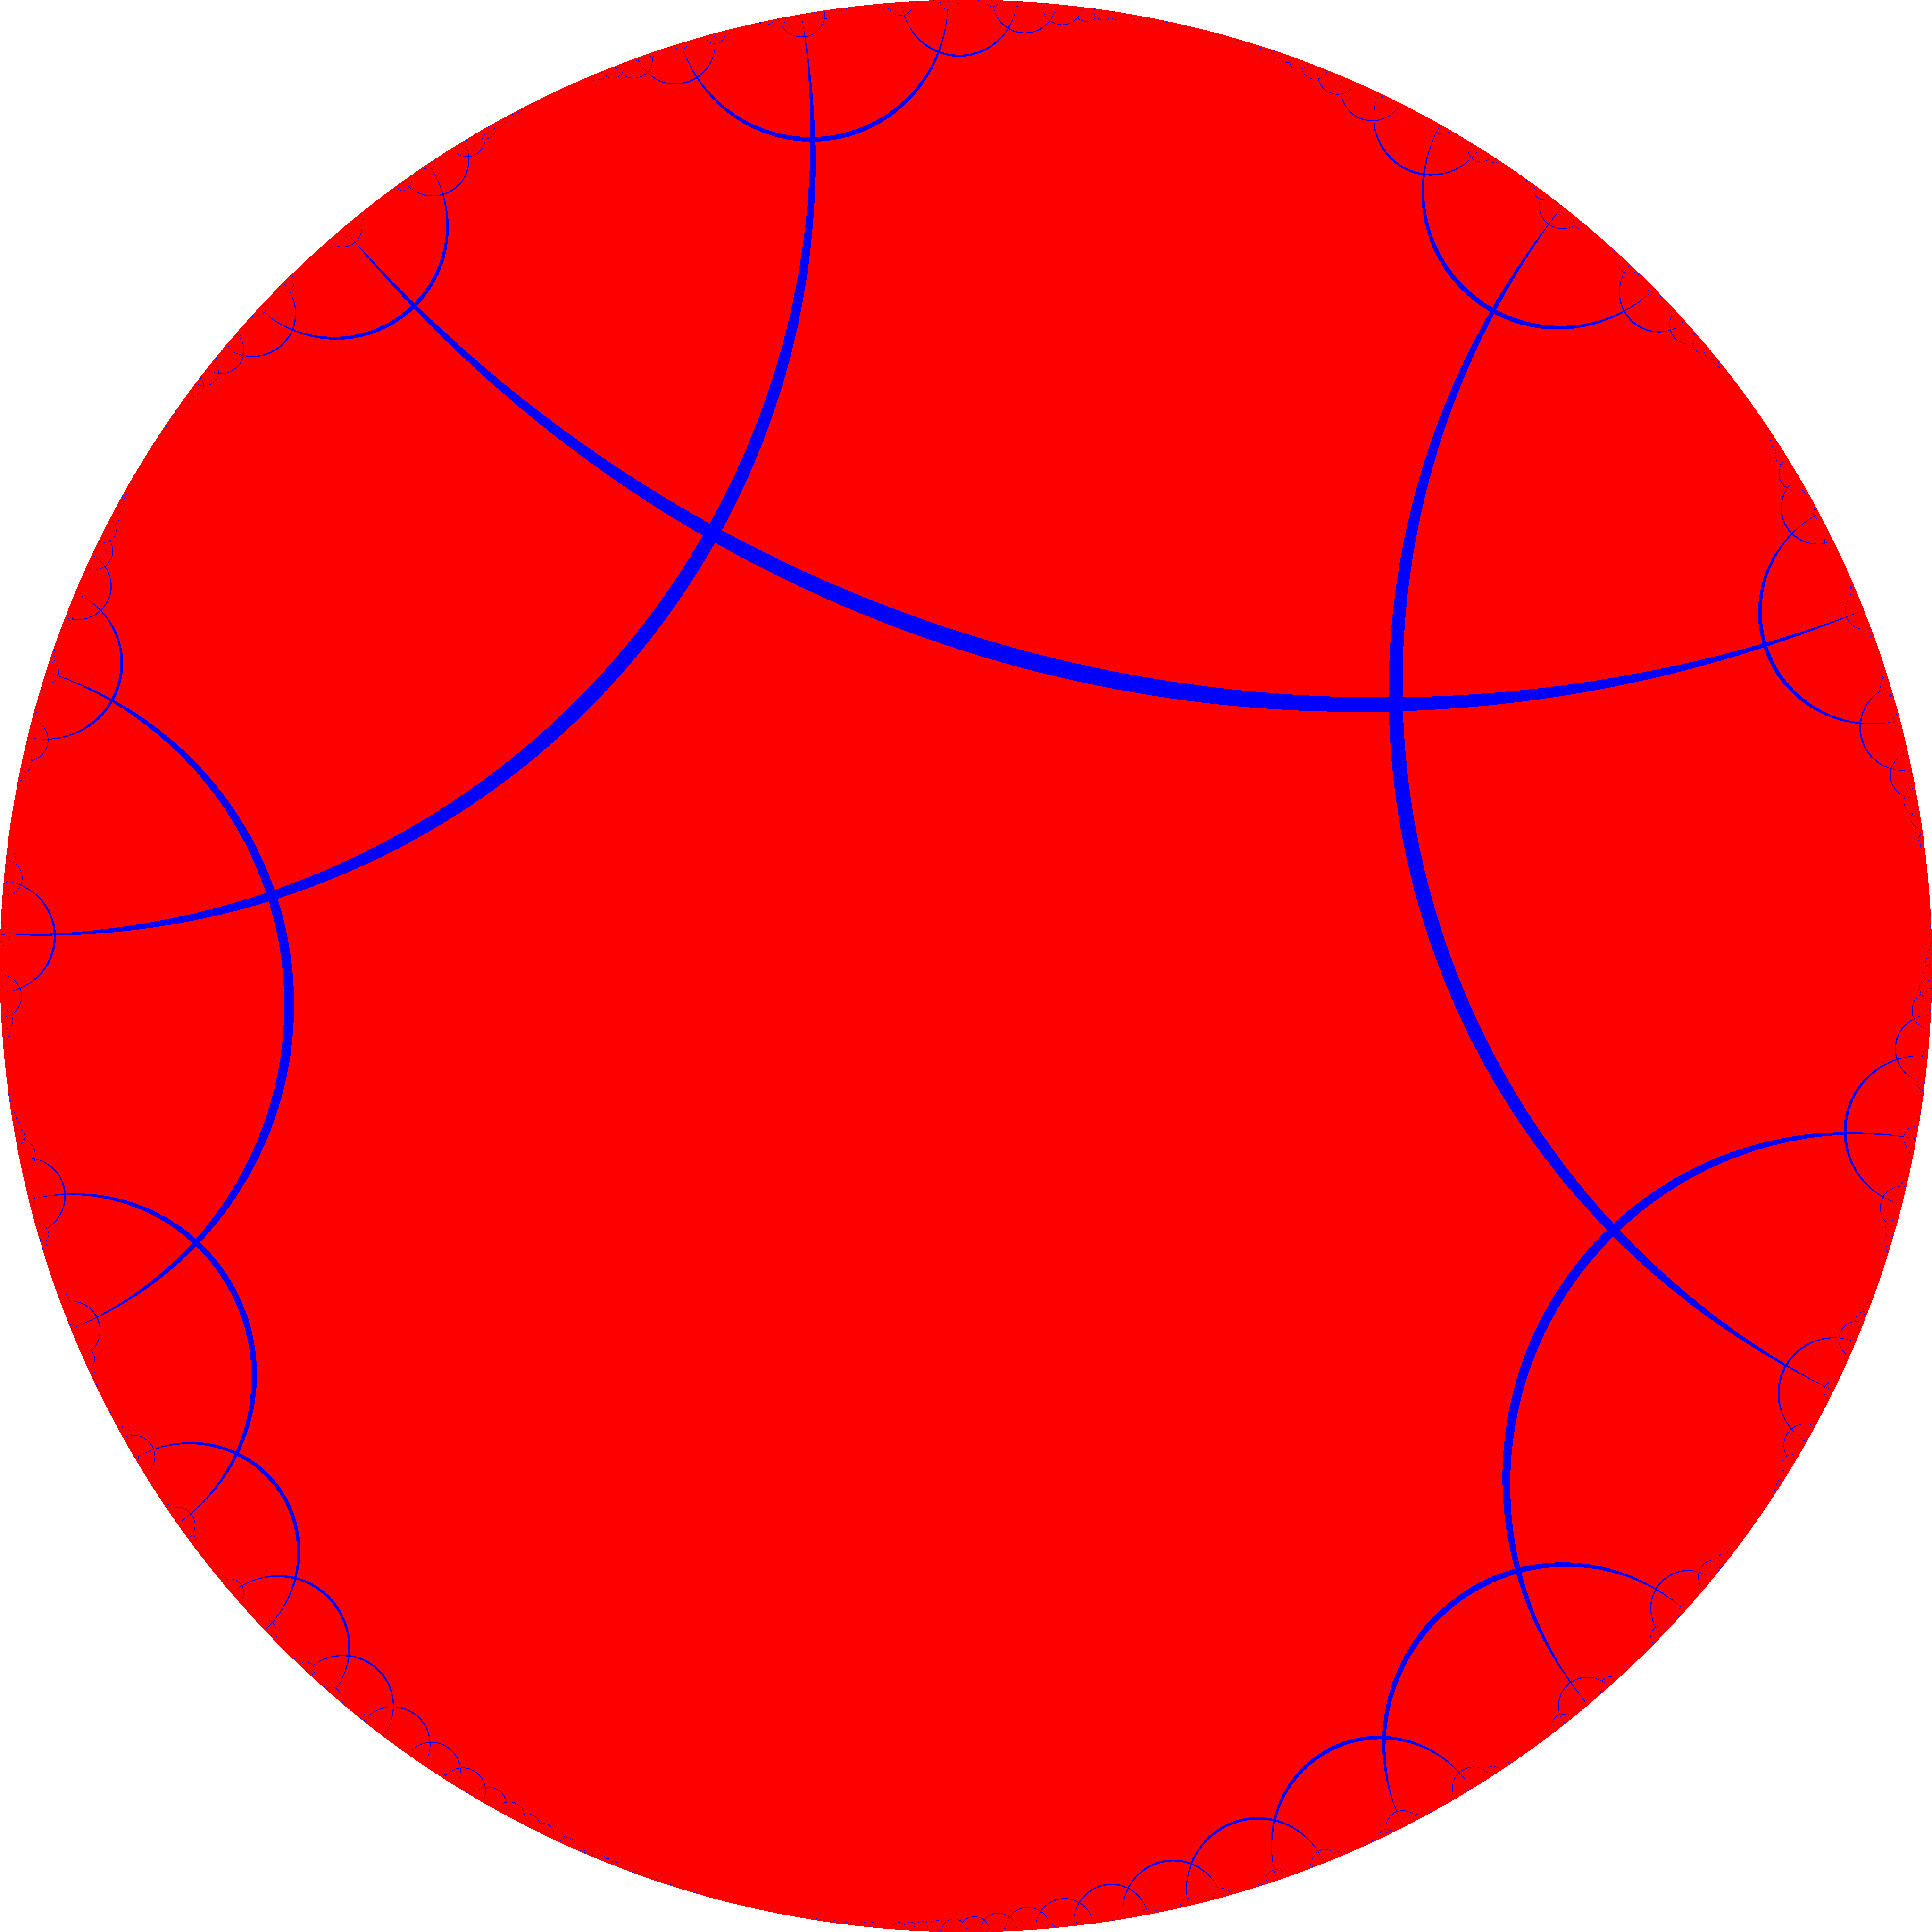
\includegraphics[width=6in]{images/t4096.png}};
    \draw (1.00, 2.60) node[inner sep=1pt] (p_z) {0};
    \draw (-3.4, +3.9) node {$-1$};
    \draw (+5.2, +1.8) node {$+1$};

    % geodesic 0 %
    \draw [black, dotted, line width=1mm]
          (-1.89, -7.39) node[inner sep=1pt] (p_pinf) {}
       -- (+1.89, +7.39) node[inner sep=1pt] (p_ninf) {};

    % geodesic 1 %
    \draw [black, dotted, line width=1mm]
          (-3.29, 6.84) arc (205.0:58.7:-2.20);

    % geodesic 1 %
    \draw [black, dotted, line width=1mm]
          (7.58, 0.55) arc (265.0:135.7:2.25);

    \draw (-0.9, +6.2) node {$-1$};
    \draw (-1.9, +2.9) node {$-\frac{1}{2}$};
    \draw (-5.0, +0.3) node {$-\frac{1}{4}$};
    \draw (-7.0, +0.0) node {$-\frac{1}{8}$};

    \draw (+3.7, +4.9) node {$+1$};
    \draw (+3.1, +1.7) node {$+\frac{1}{2}$};
    \draw (+5.2, -2.5) node {$+\frac{1}{4}$};
\end{tikzpicture}
\caption{嵌入 $n$ 线}
\end{figure}

上图中的黑线是我们恰当连接无穷远点得到的,随着 $-1$ 和 $+1$ 的出现,全体整数都出现在我们的开始寻找零点的那条加线上。
这样我们就完成了嵌入 $n$ 的任务。

\newpage

\subsection{嵌入$2^{-n}$}

寻找恰当的 $+\frac{1}{2}$ 点。

\newpage

\subsection{嵌入$1 - 2^{-n}$}

寻找恰当的 $+\frac{3}{2}$ 点。

\newpage

\subsection{嵌入$1 + 2^{-n}$}

\newpage

\section{嵌入超现实数的证明}

上面的构造过程蕴含了共形嵌入的证明思路,在此我们给出严格的证明。

\subsection{证明的主体}

\subsection{推论:黎曼共形映射定理}

核心的几何想法:

复平面上的任意简单连通的闭曲线 $C$,我们可以构造一个圆盘包含它,然后把圆盘视为庞加莱圆盘。

这时候超现实数嵌入在这个庞加莱圆盘里,我们有先序遍历超现实数的得到的一条路径,它类似平面上的希尔伯特曲线,不妨也命名为 $H$。

我们考察闭曲线和曲线 $H$ 的交点,我们沿着希尔伯特曲线的奇数步(或者偶数步)的这些折线向外展开,就能把交点送到无穷远。

注意到$H$上,所有奇数步的线都是彼此平行的(非常可能是等值线),它们能把 $C$ 自然地光滑映射到庞加莱圆盘的边缘。

\newpage

\section{环与扩域的想法}

\subsection{基础元素}

$\begin{array}{|c|c|}\hline 1&\space\\\hline n&0\\\hline\end{array} \mapsto n$ 代表整数,整个树都是整数值 $n$

$\begin{array}{|c|c|}\hline0&\space\\\hline 1&0\\\hline\end{array} \mapsto h$ 代表全体横向测地线(加线)的过滤器

$\begin{array}{|c|c|}\hline0&\space\\\hline 0&1\\\hline\end{array} \mapsto i$ 代表全体横向测地线(加线)上的自然增加

$\begin{array}{|c|c|}\hline2&\space\\\hline 1&0\\\hline\end{array} \mapsto j$ 代表全体纵向测地线(乘线)上的自然增加

$\begin{array}{|c|c|}\hline2&\space\\\hline 0&1\\\hline\end{array} \mapsto q$

$p$ 是将 $q$ 的加乘位置互易得到

\subsubsection{问题}

$o_p$ 独点的过滤器存在吗?其中 $p$ 是从原点到达该点路径的二进制编码

$g_p$ 单独一条测地线的过滤器存在吗?其中 $p$ 是从原点到达测地线的路径的二进制编码

$n$ 自己可以构成域,$n$ 与 $q$ 的组合能生成域吗?$n$ 与 $p$、 $q$ 的组合能生成域吗?

生成域的目标是包含 surreal number。

\subsection{$i$ 上的结构}

\subsubsection{加线和所有的倍加线}

\subsubsection{边界上的希尔伯特空间}

对于庞加莱圆盘和边界,其实边界不应该看成一条线,正确的几何观点是看成无数条彼此垂直的测地线在边界捏合起来,这些测地线构成希尔伯特空间。

\newpage

\section{几个研究的方向}

任何一个程序化的计算过程体现为 $\mathfrak{K}$ 上的一个流动。

1、初等数学:用函数式的观点,理解计算流动过程,重新考察初等几何、线性代数、微积分和微分方程等。比如圆是什么?线性是非常值得考察的。

2、计算理论:Chaitin 常数 $\Omega$ 的几何位置在哪里?

4、优化与变分:重新考察优化与变分,前传、后传。重要的是,大自然本身是优化过程,拉氏量的最小化。

5、学习理论:学习过程体现为一个反复迭代的程序,是测地线上的流动,重新考察学习的概念。

6、几何学:对于一个计算过程,是否存在一个观察角度使得计算流动保持体积不变?$\mathfrak{K}$上的保体积流和测地线流的研究会带来什么?


\end{document}
